% !TEX root = ../report.tex
\section*{Techniques}\label{sec:techniques}
\addcontentsline{toc}{section}{Techniques}

\begin{figure}[H]
	\subfloat[]{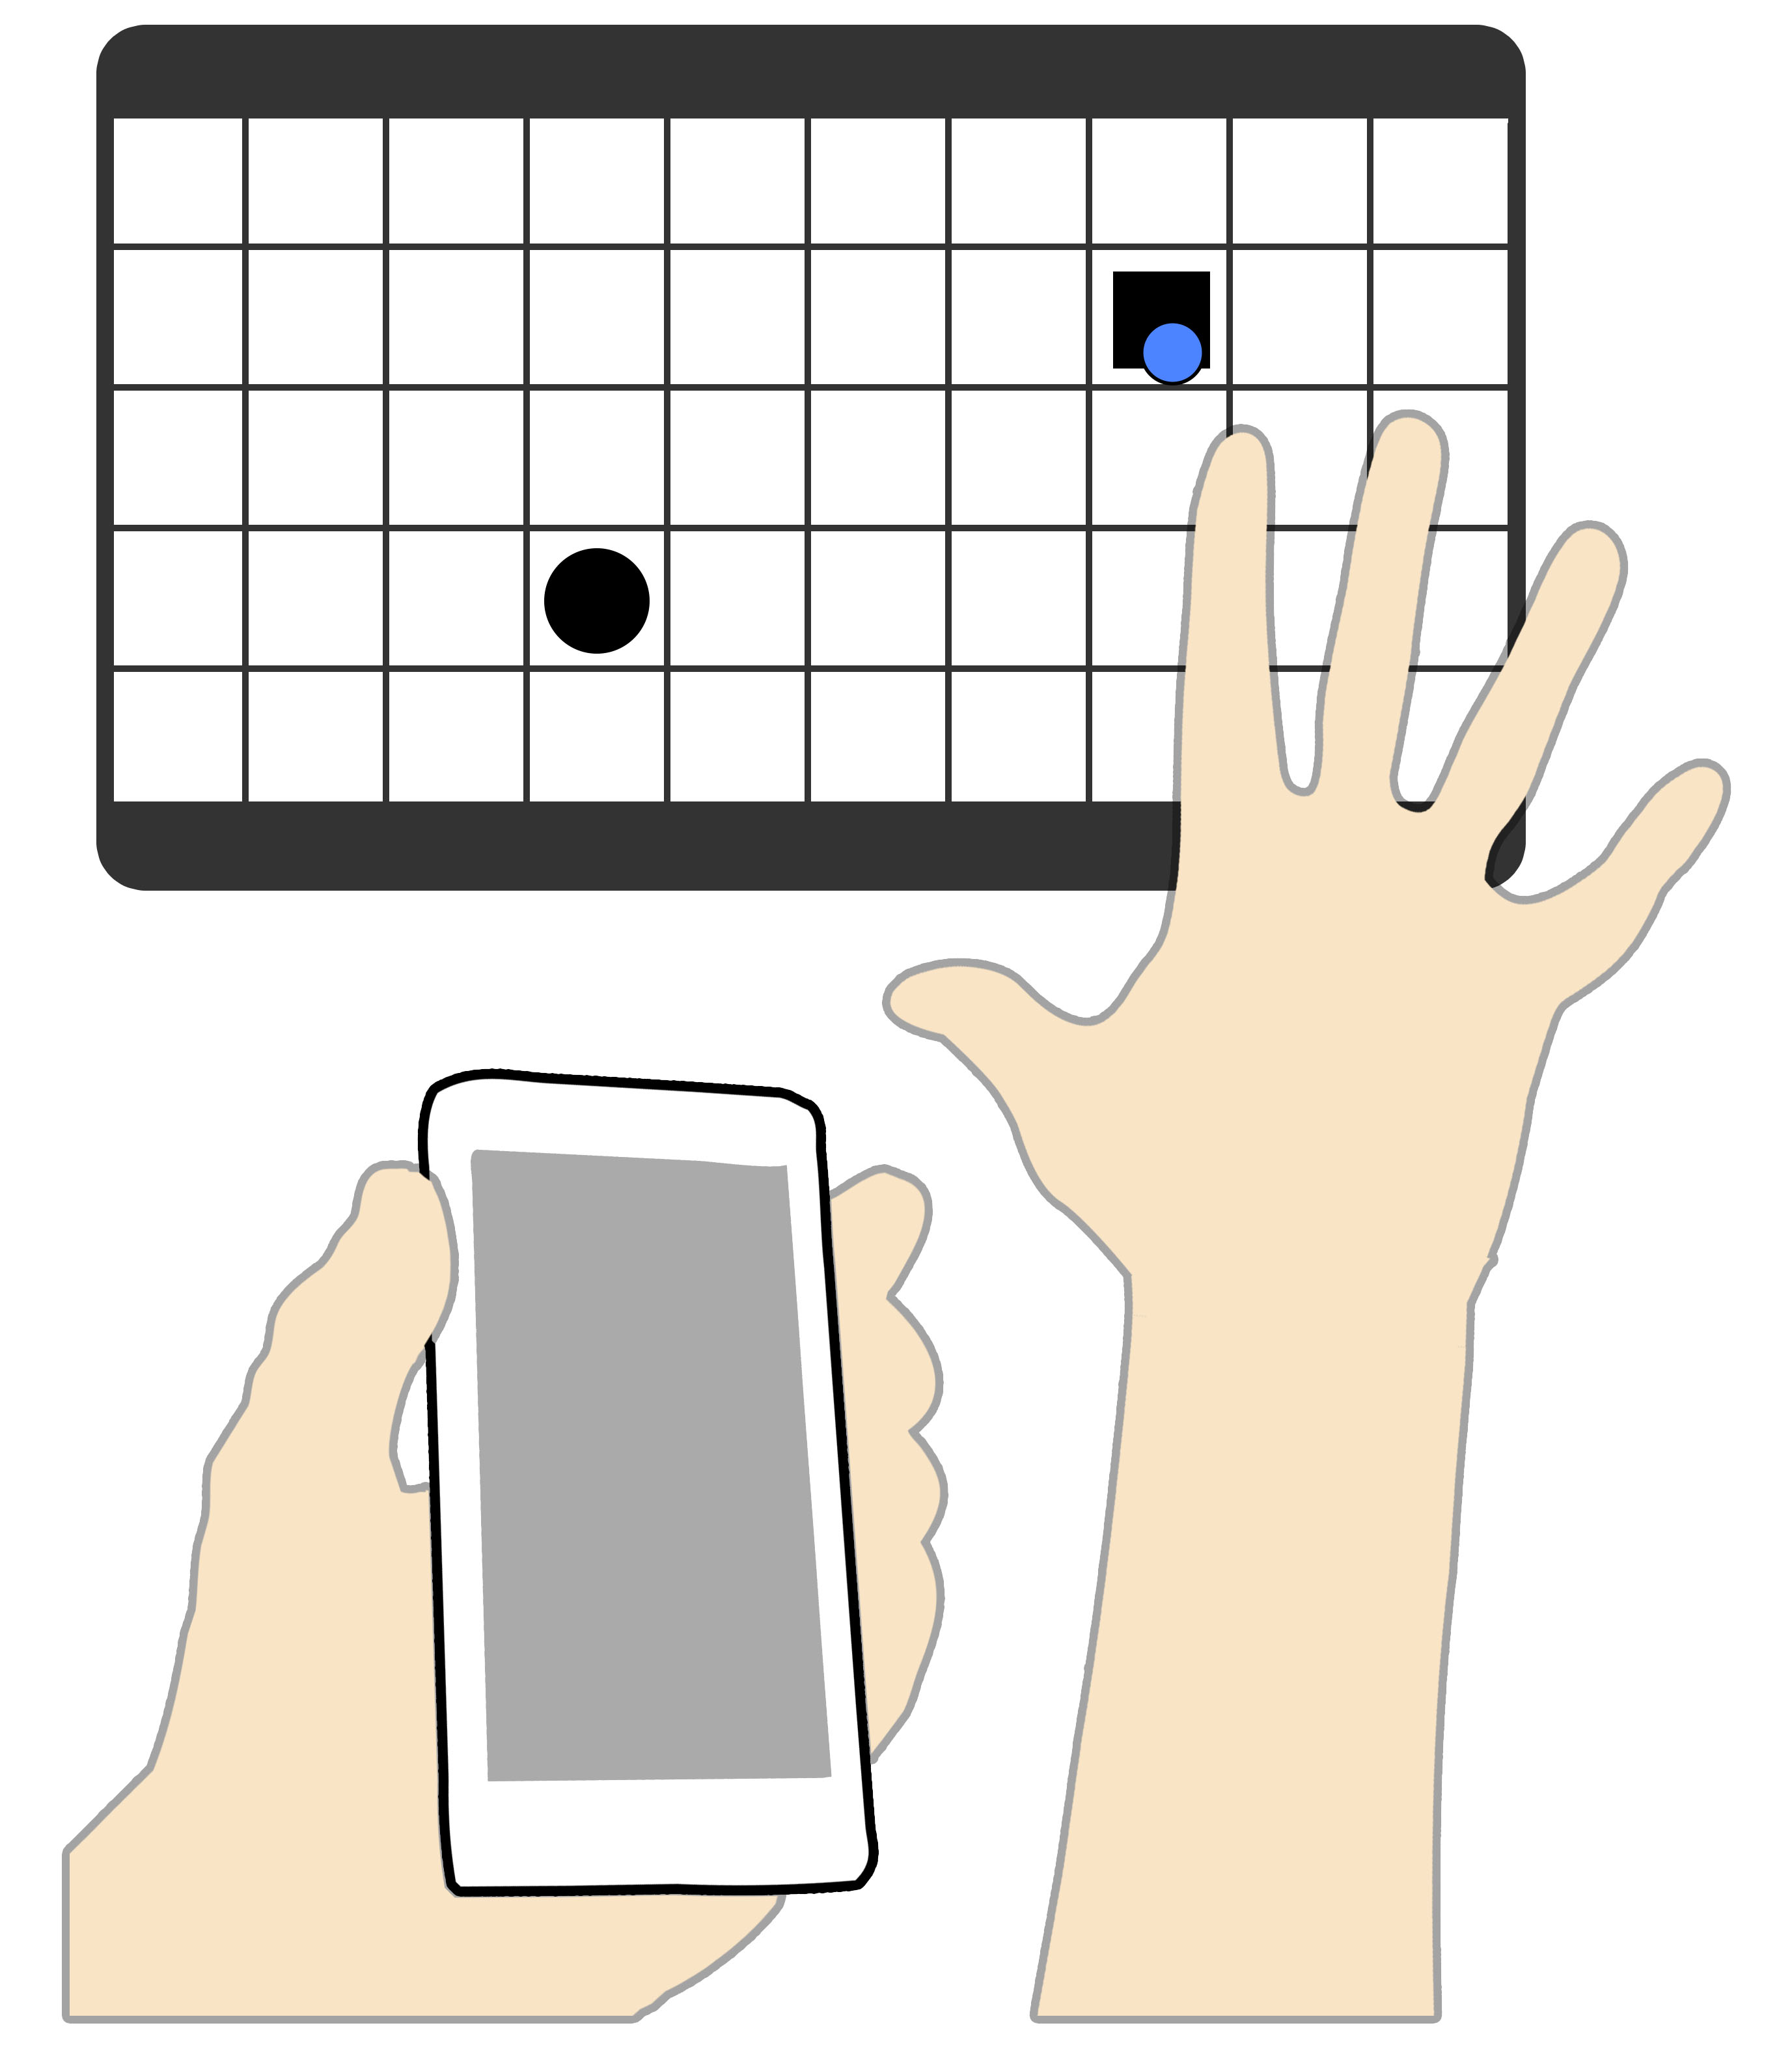
\includegraphics[width = 0.33\columnwidth]{images/techniques/grabPull1.jpg}\label{fig:grabPull1}}
	\subfloat[]{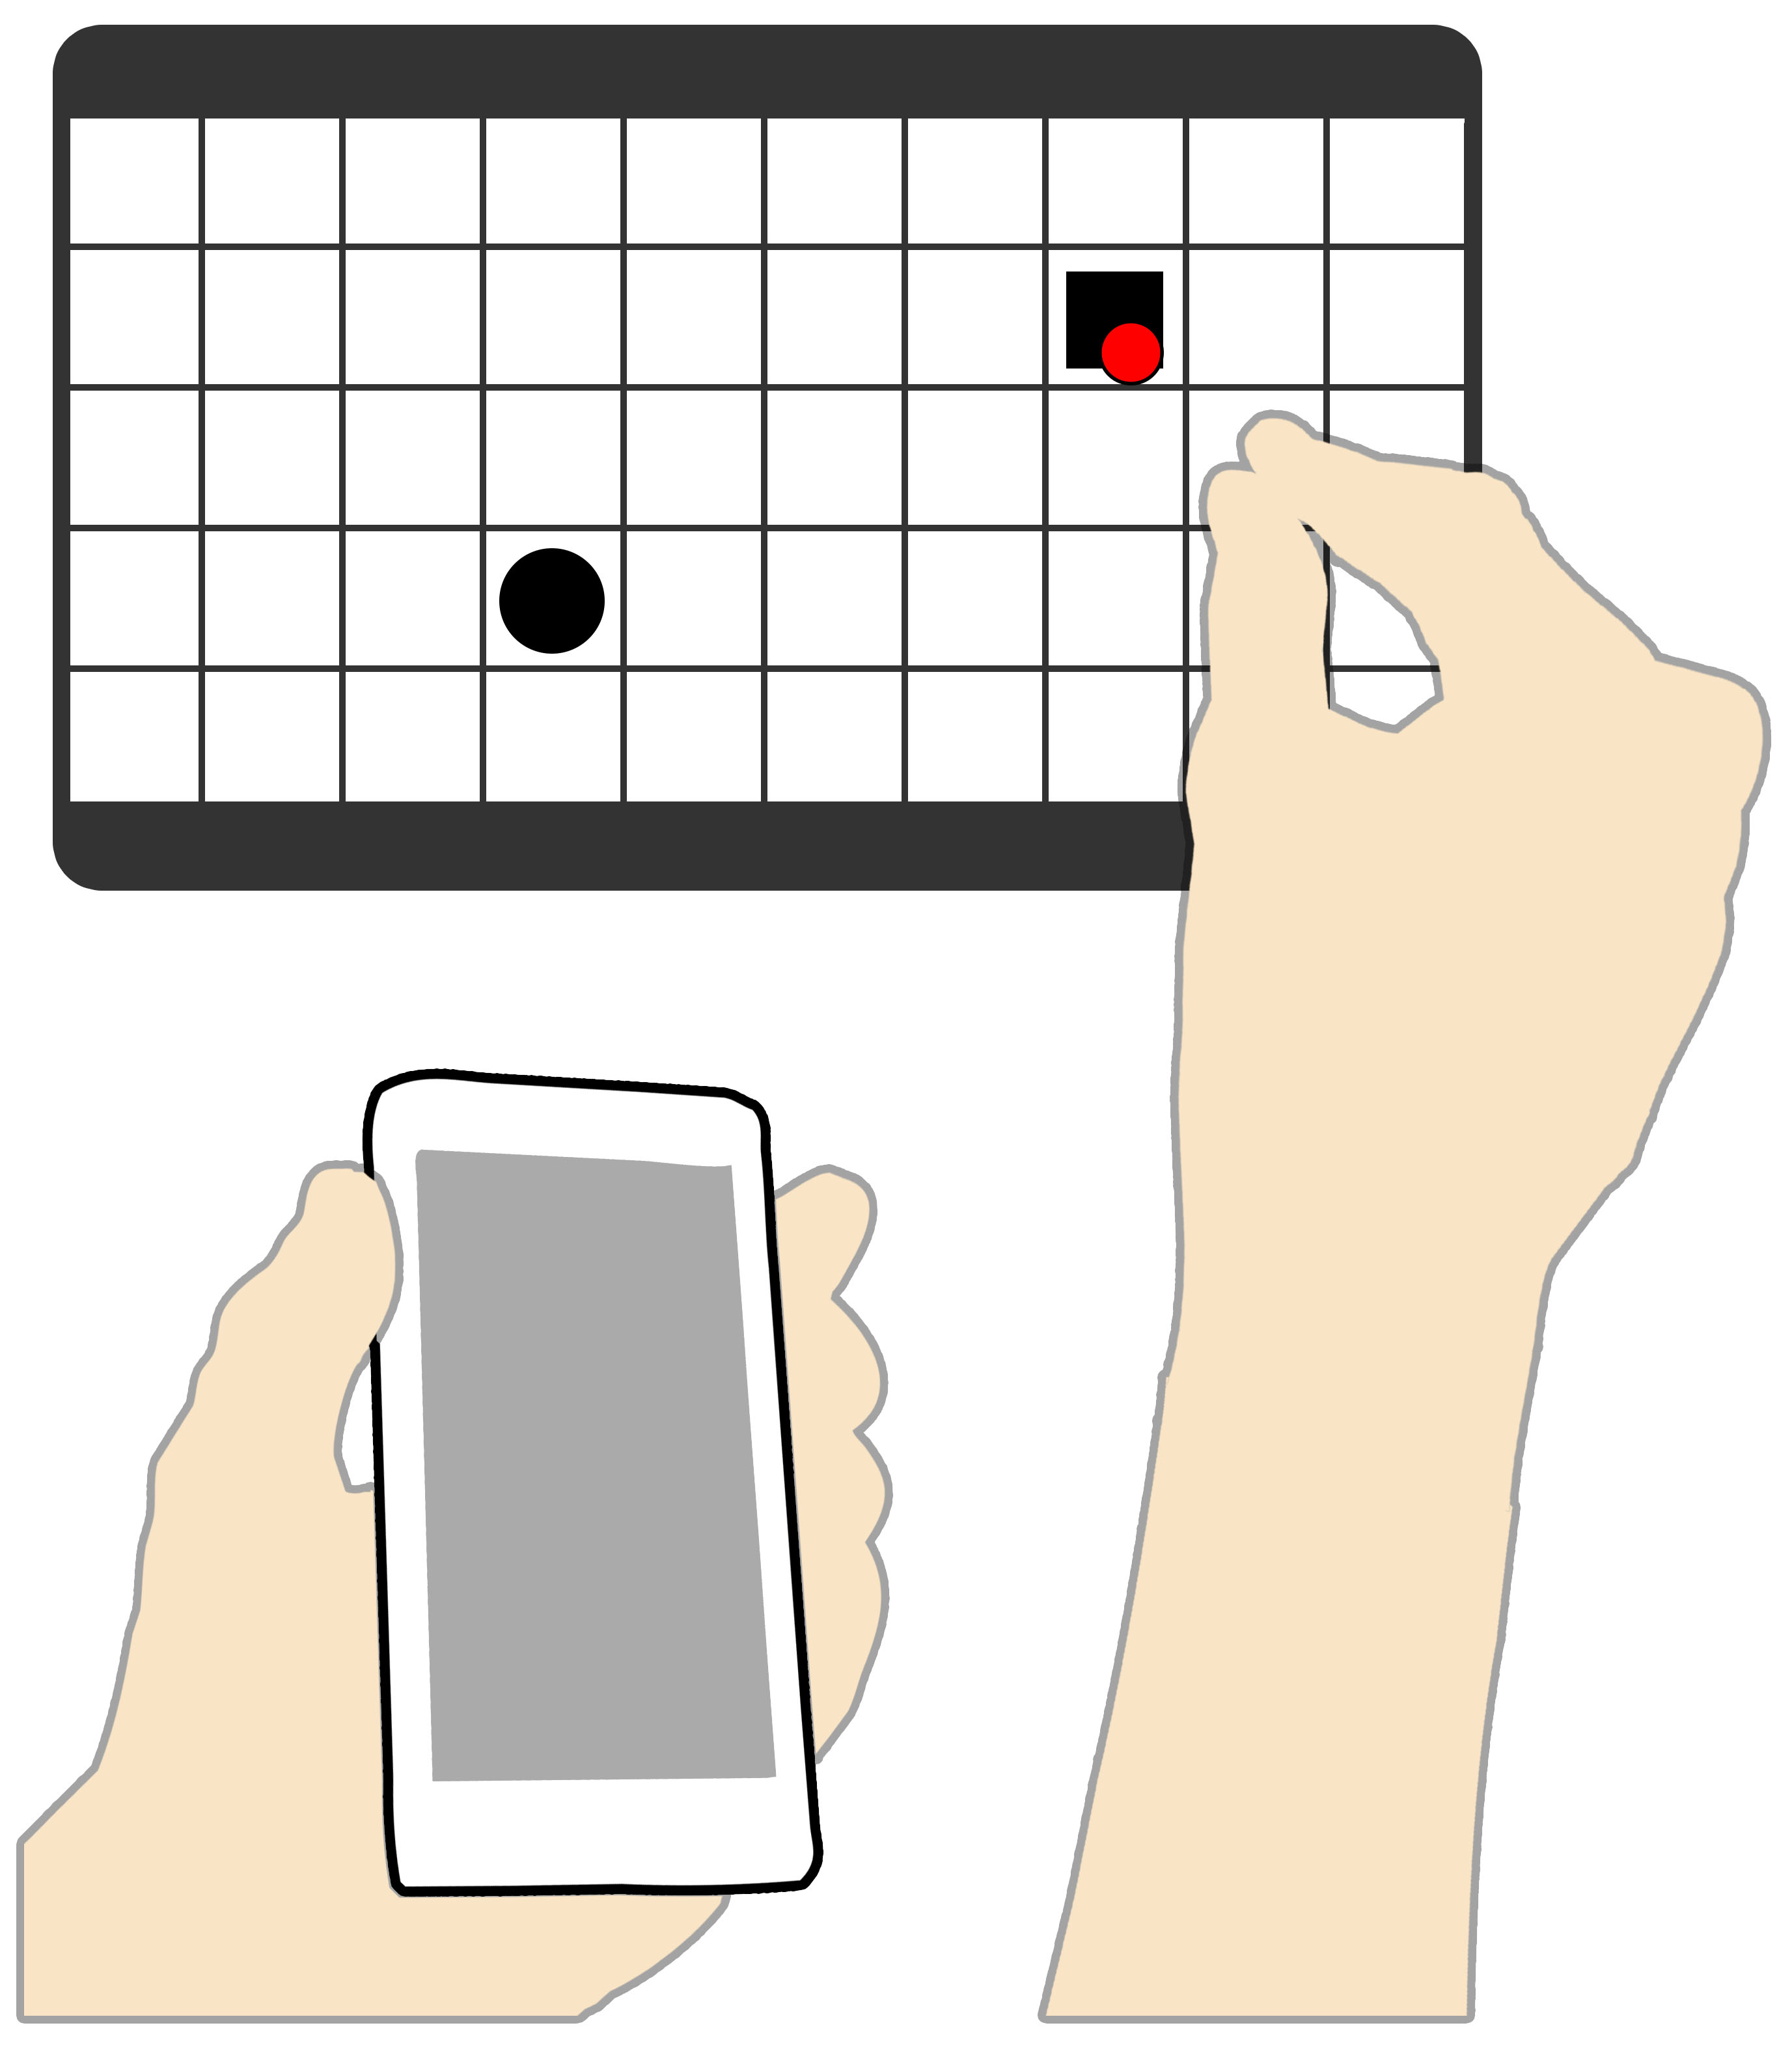
\includegraphics[width = 0.33\columnwidth]{images/techniques/grabPull2.jpg}\label{fig:grabPull2}}
	\subfloat[]{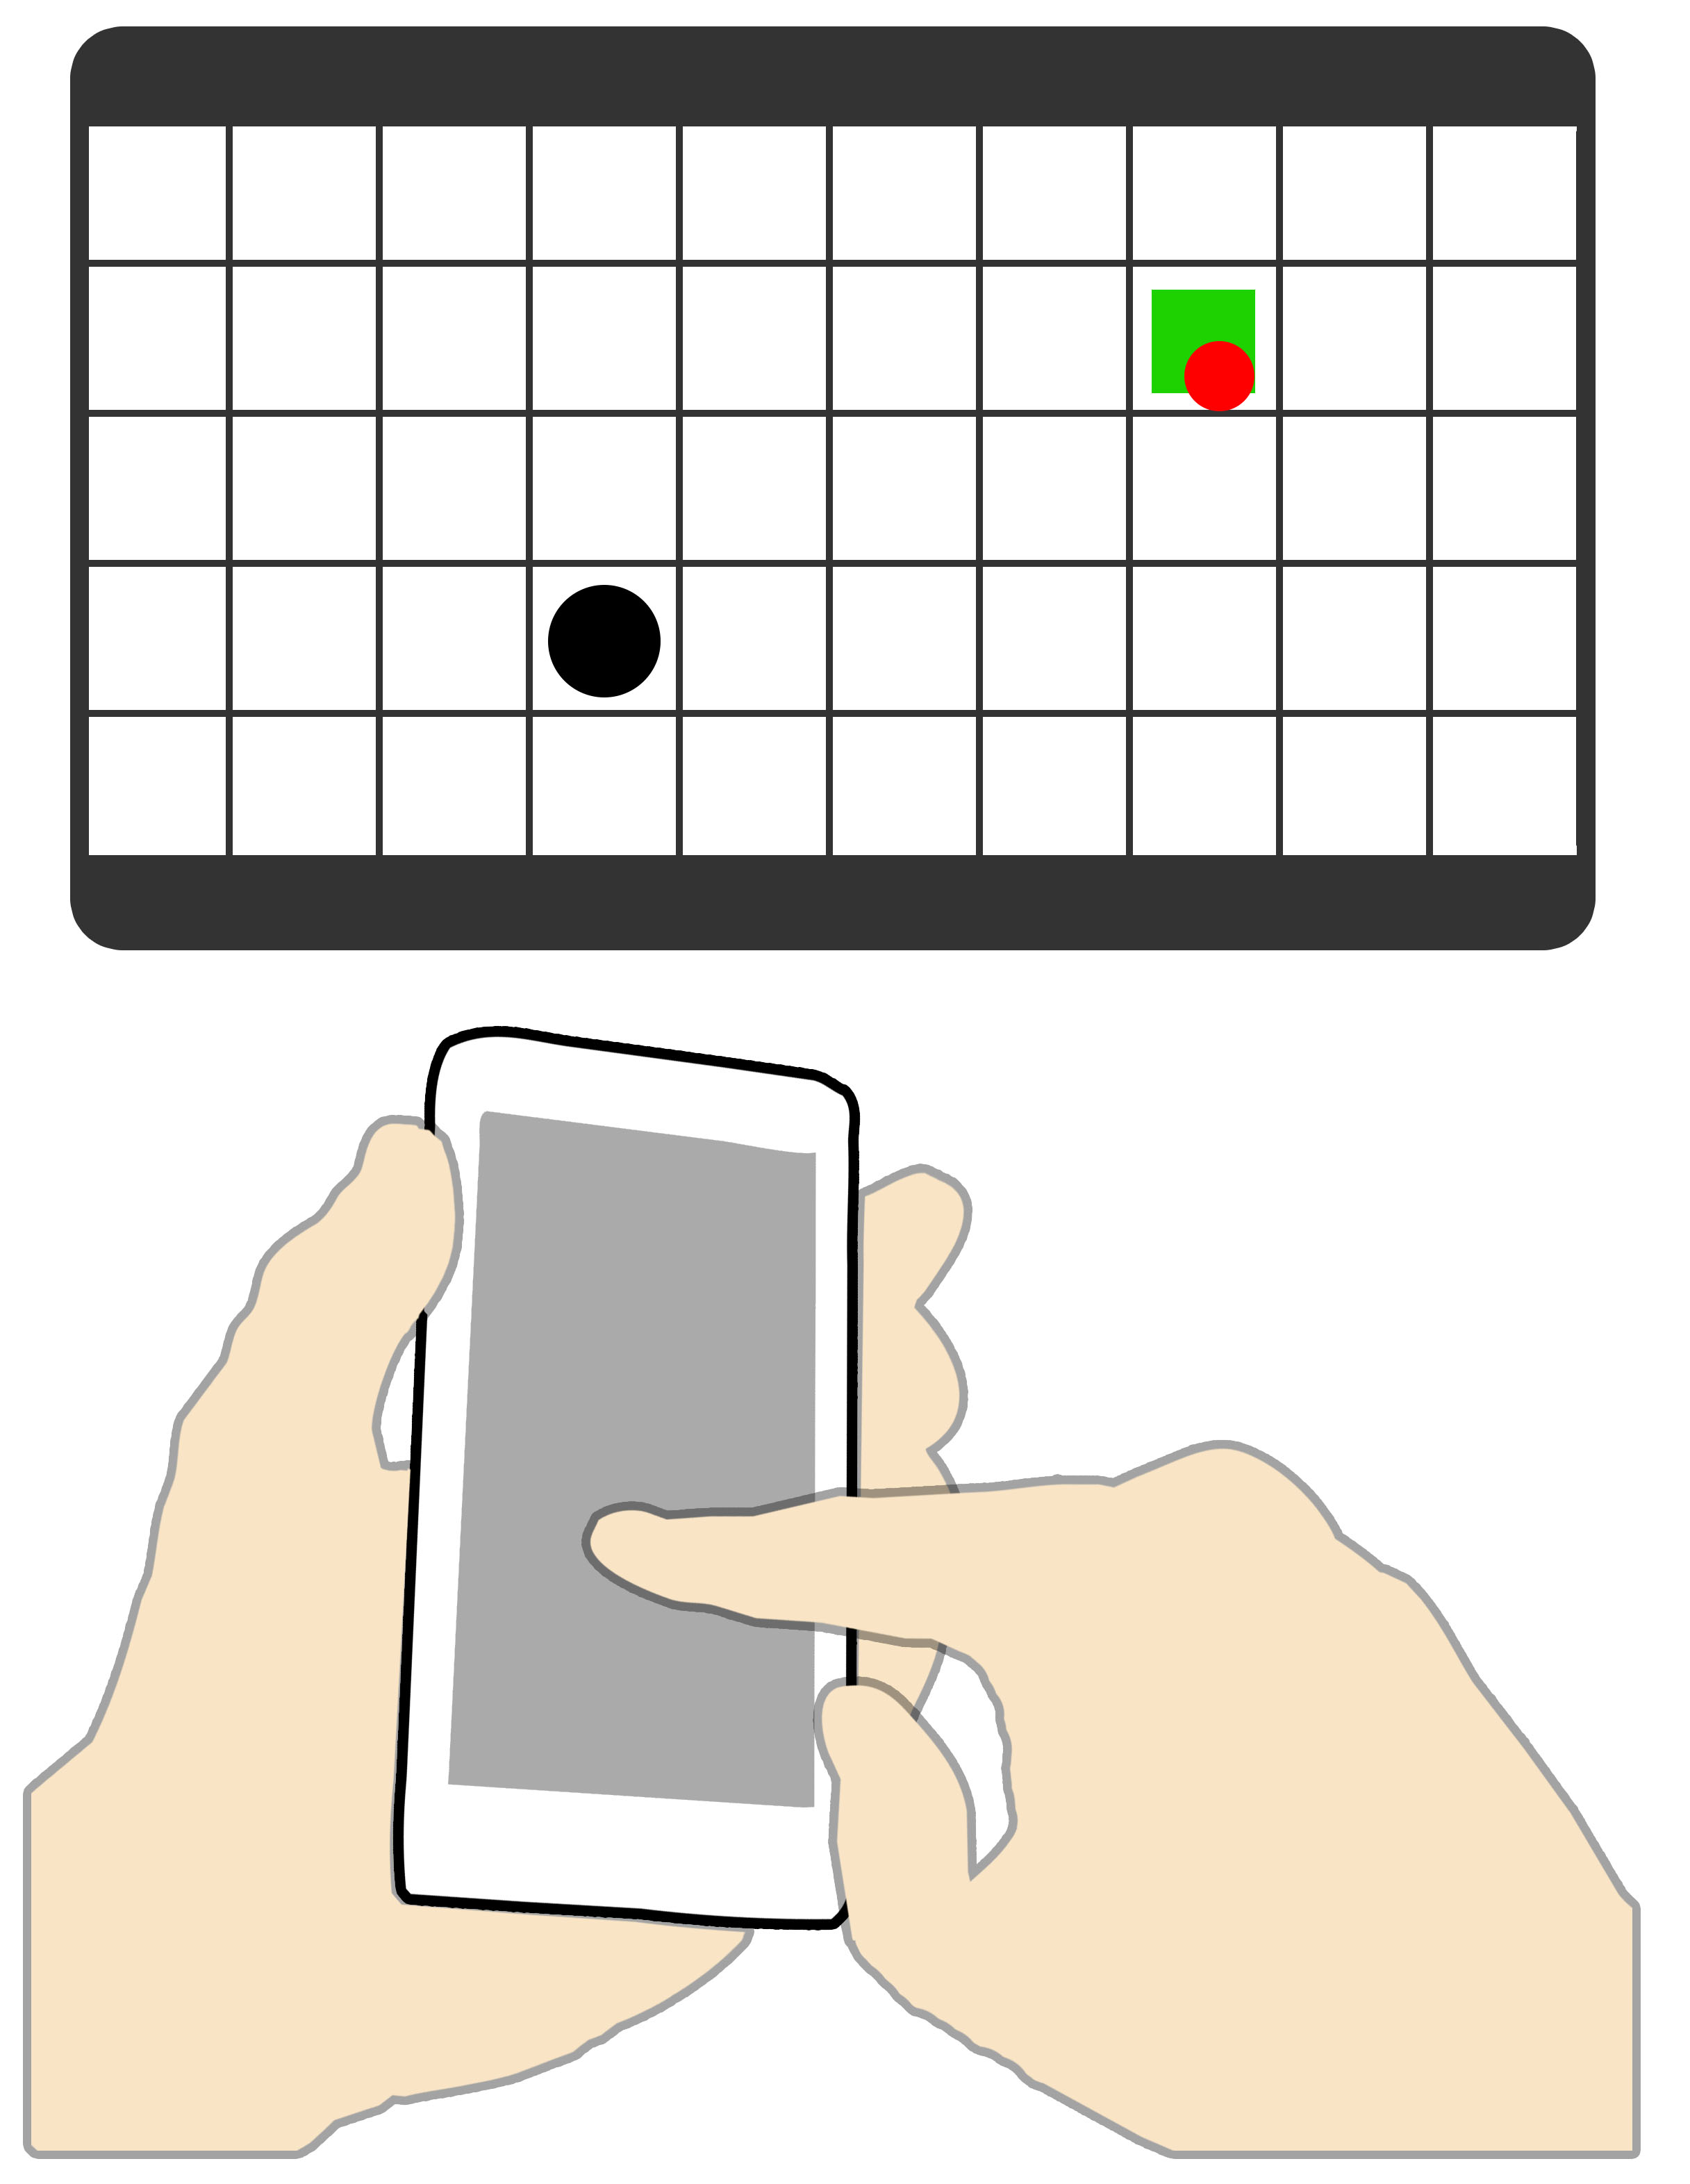
\includegraphics[width = 0.33\columnwidth]{images/techniques/grabPull3.jpg}\label{fig:grabPull3}}
	\caption{Pull grab technique}
	\label{fig:grabTechnique}
\end{figure}

\begin{figure}[H]
	\subfloat[]{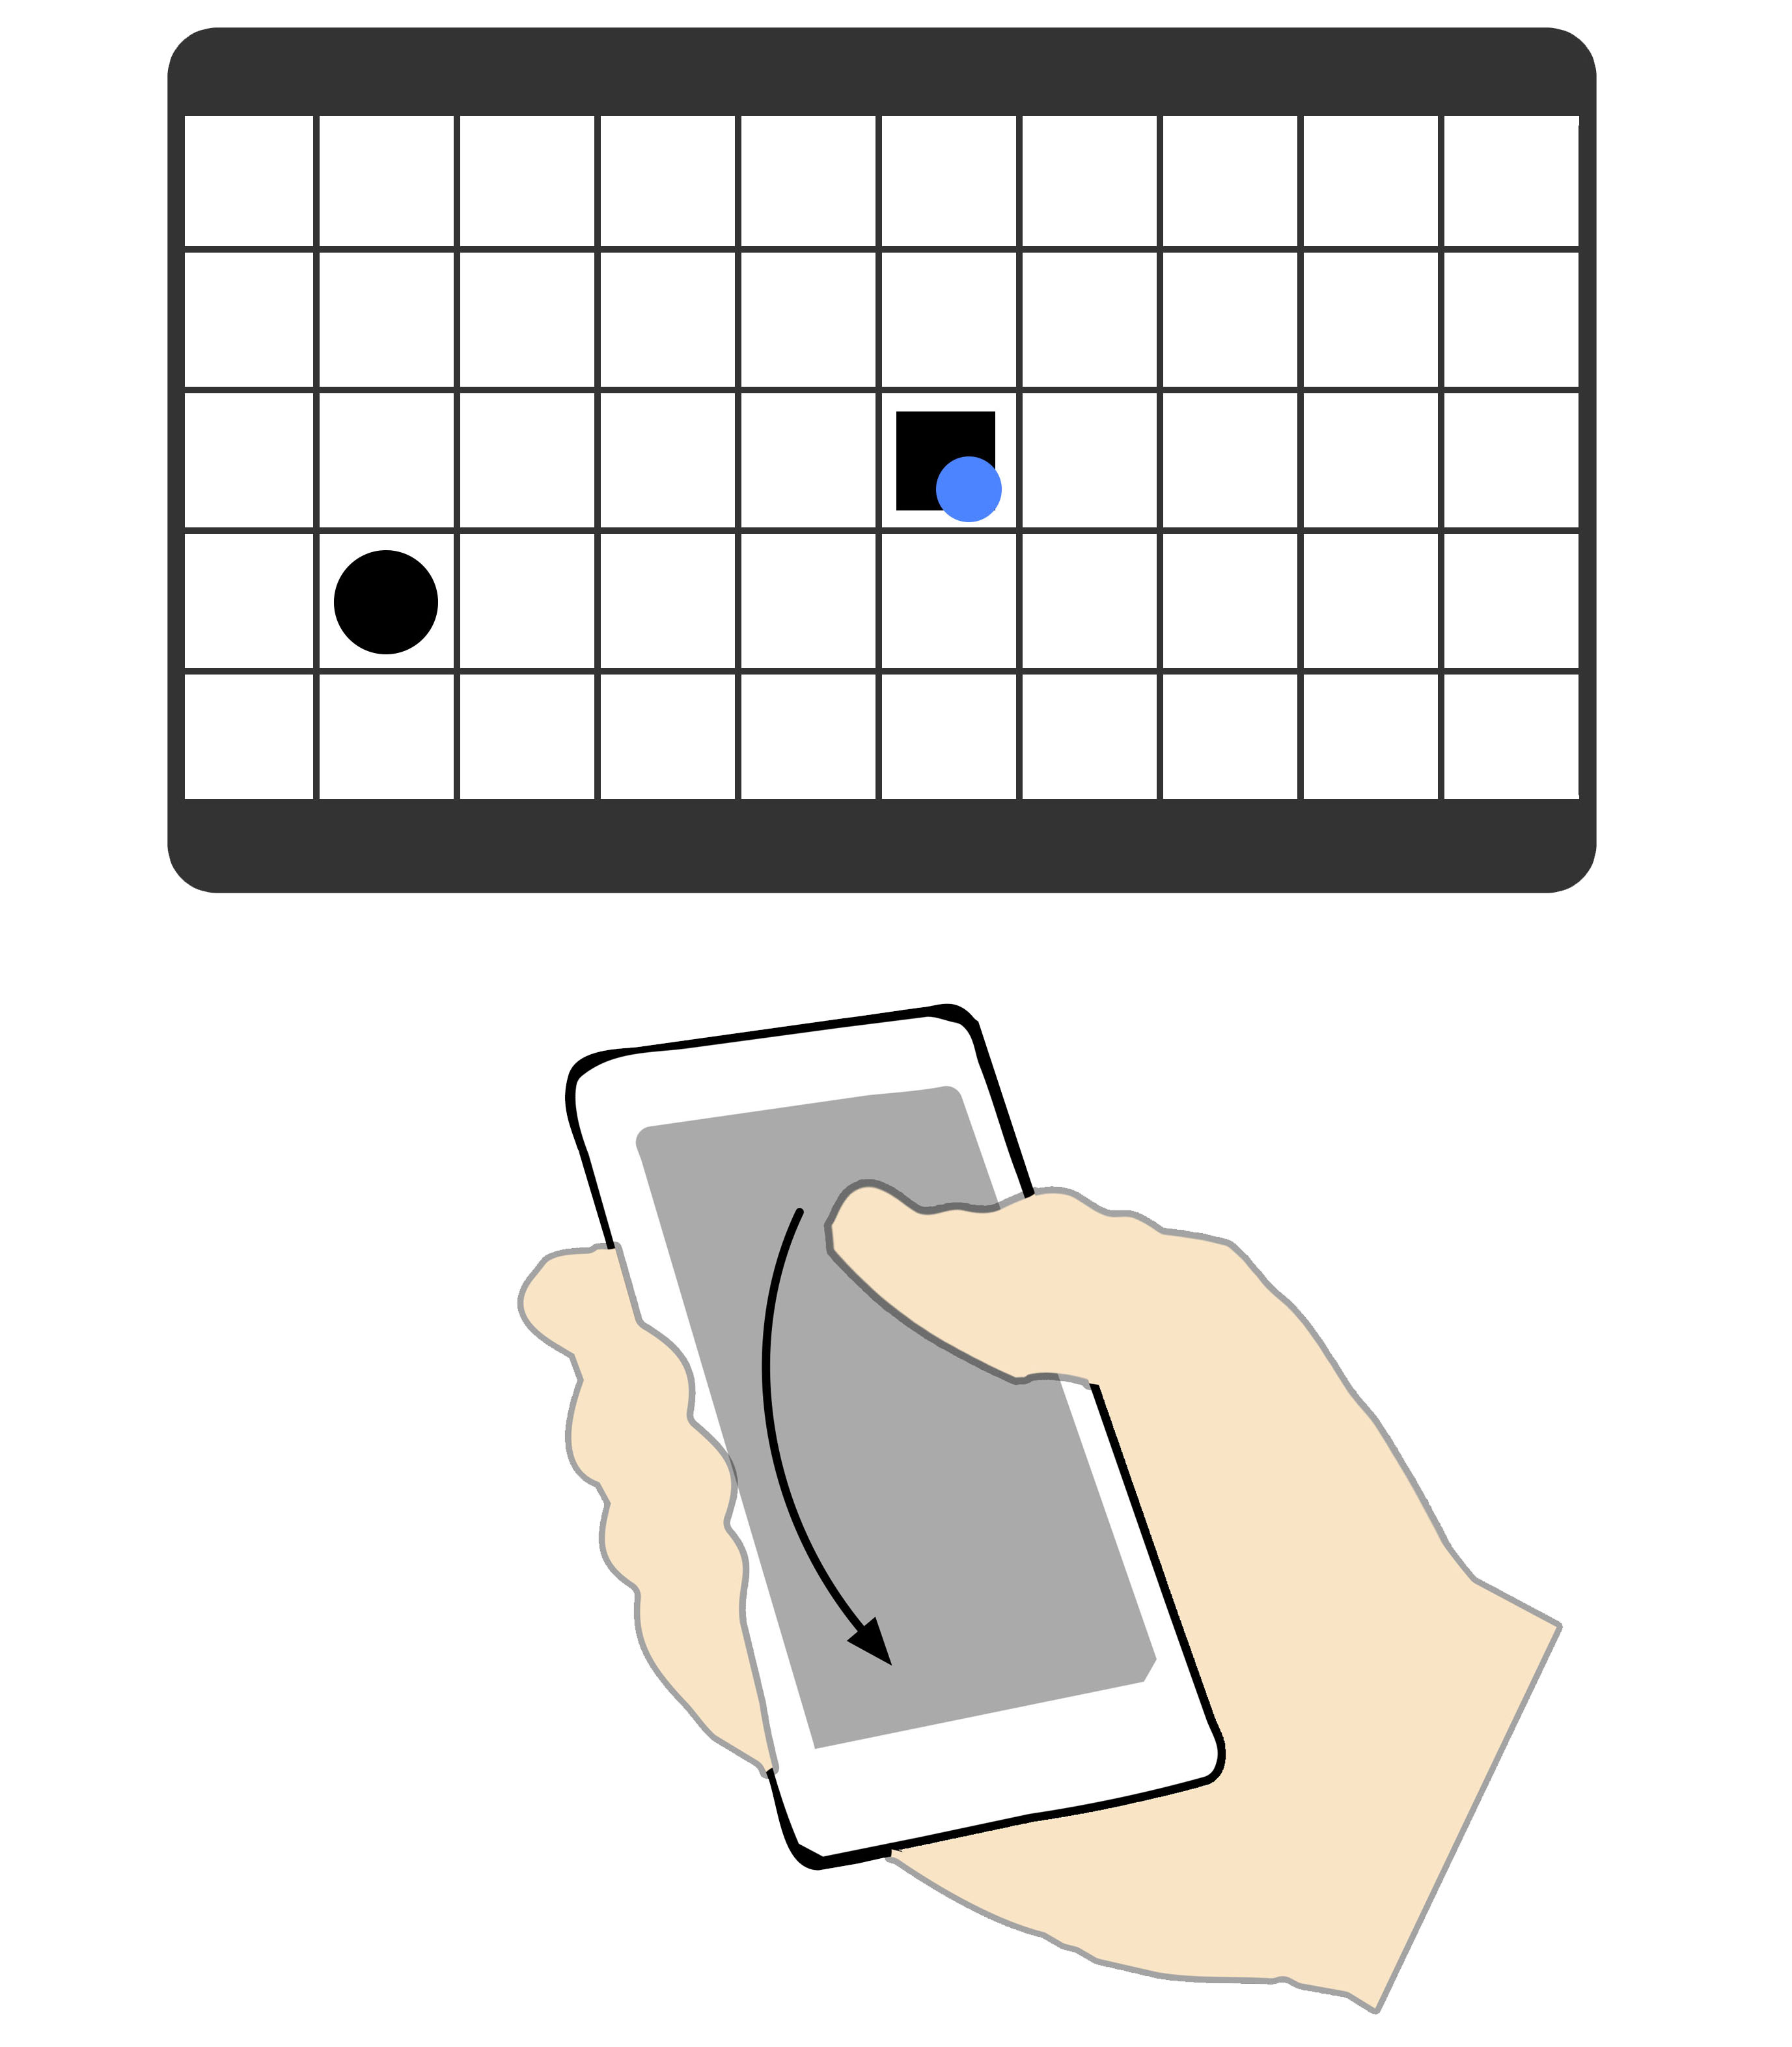
\includegraphics[width = 0.33\columnwidth]{images/techniques/swipePull1.jpg}\label{fig:swipePull1}}
	\subfloat[]{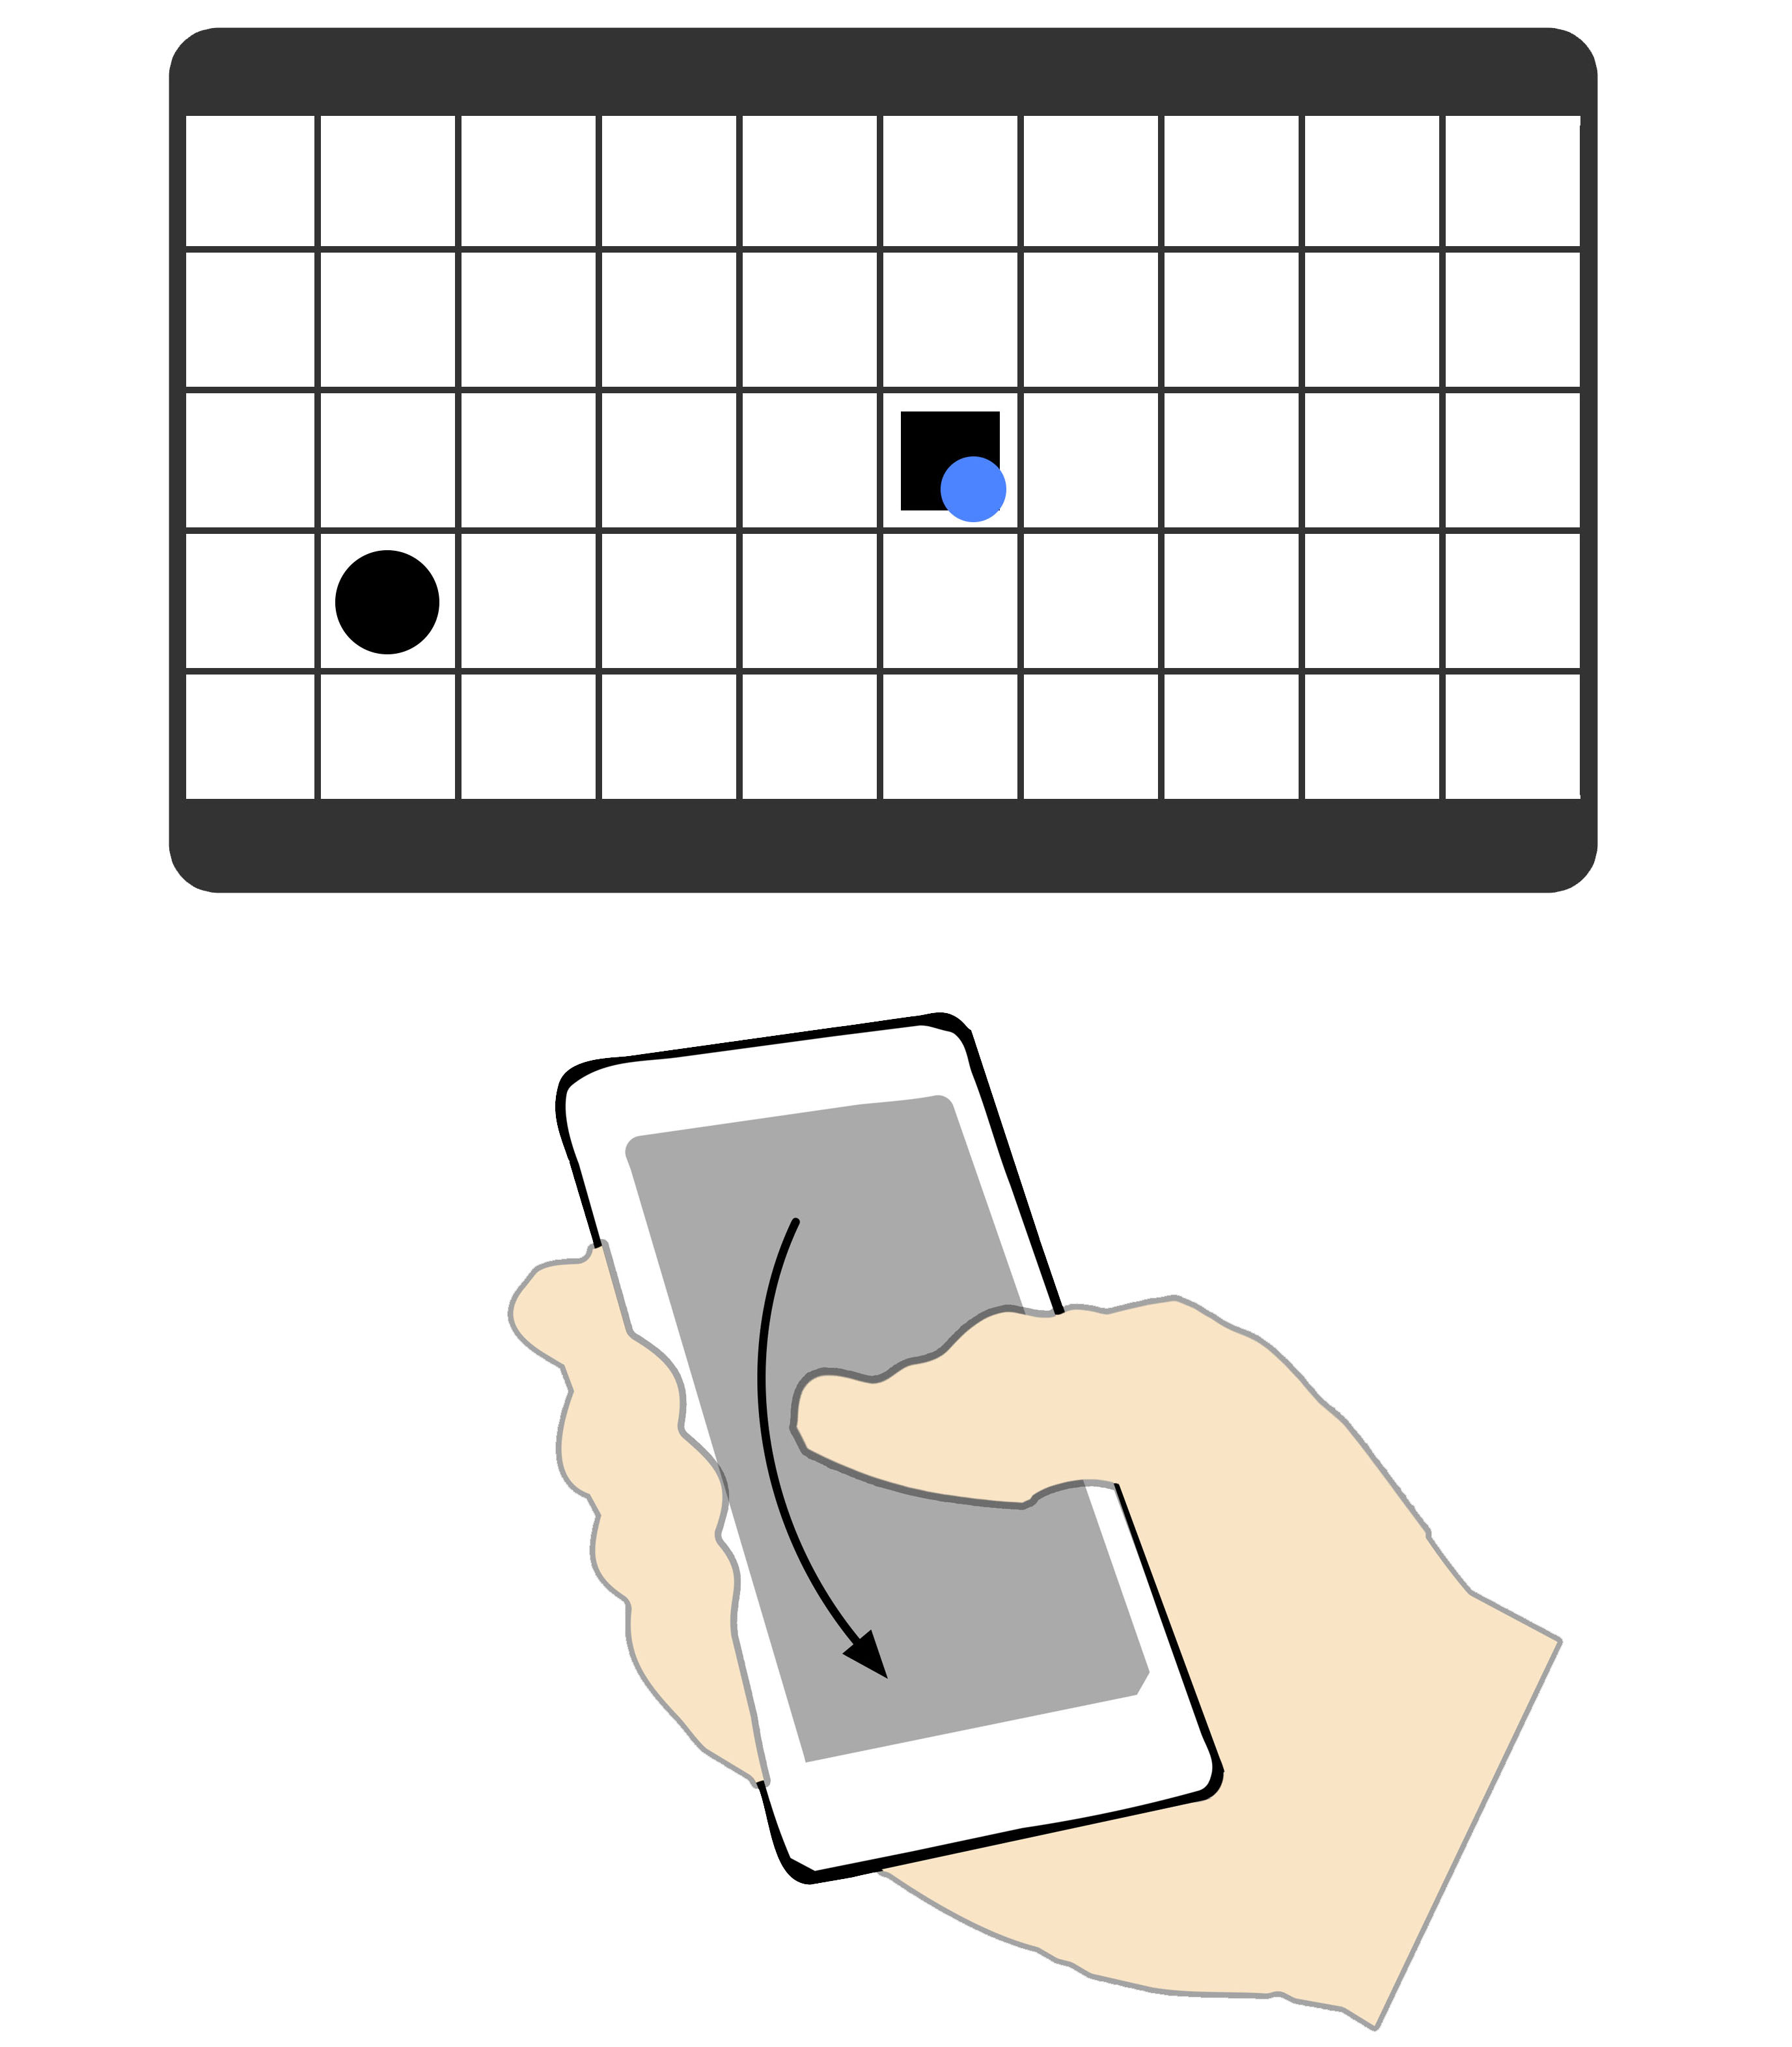
\includegraphics[width = 0.33\columnwidth]{images/techniques/swipePull2.jpg}\label{fig:swipePull2}}
	\subfloat[]{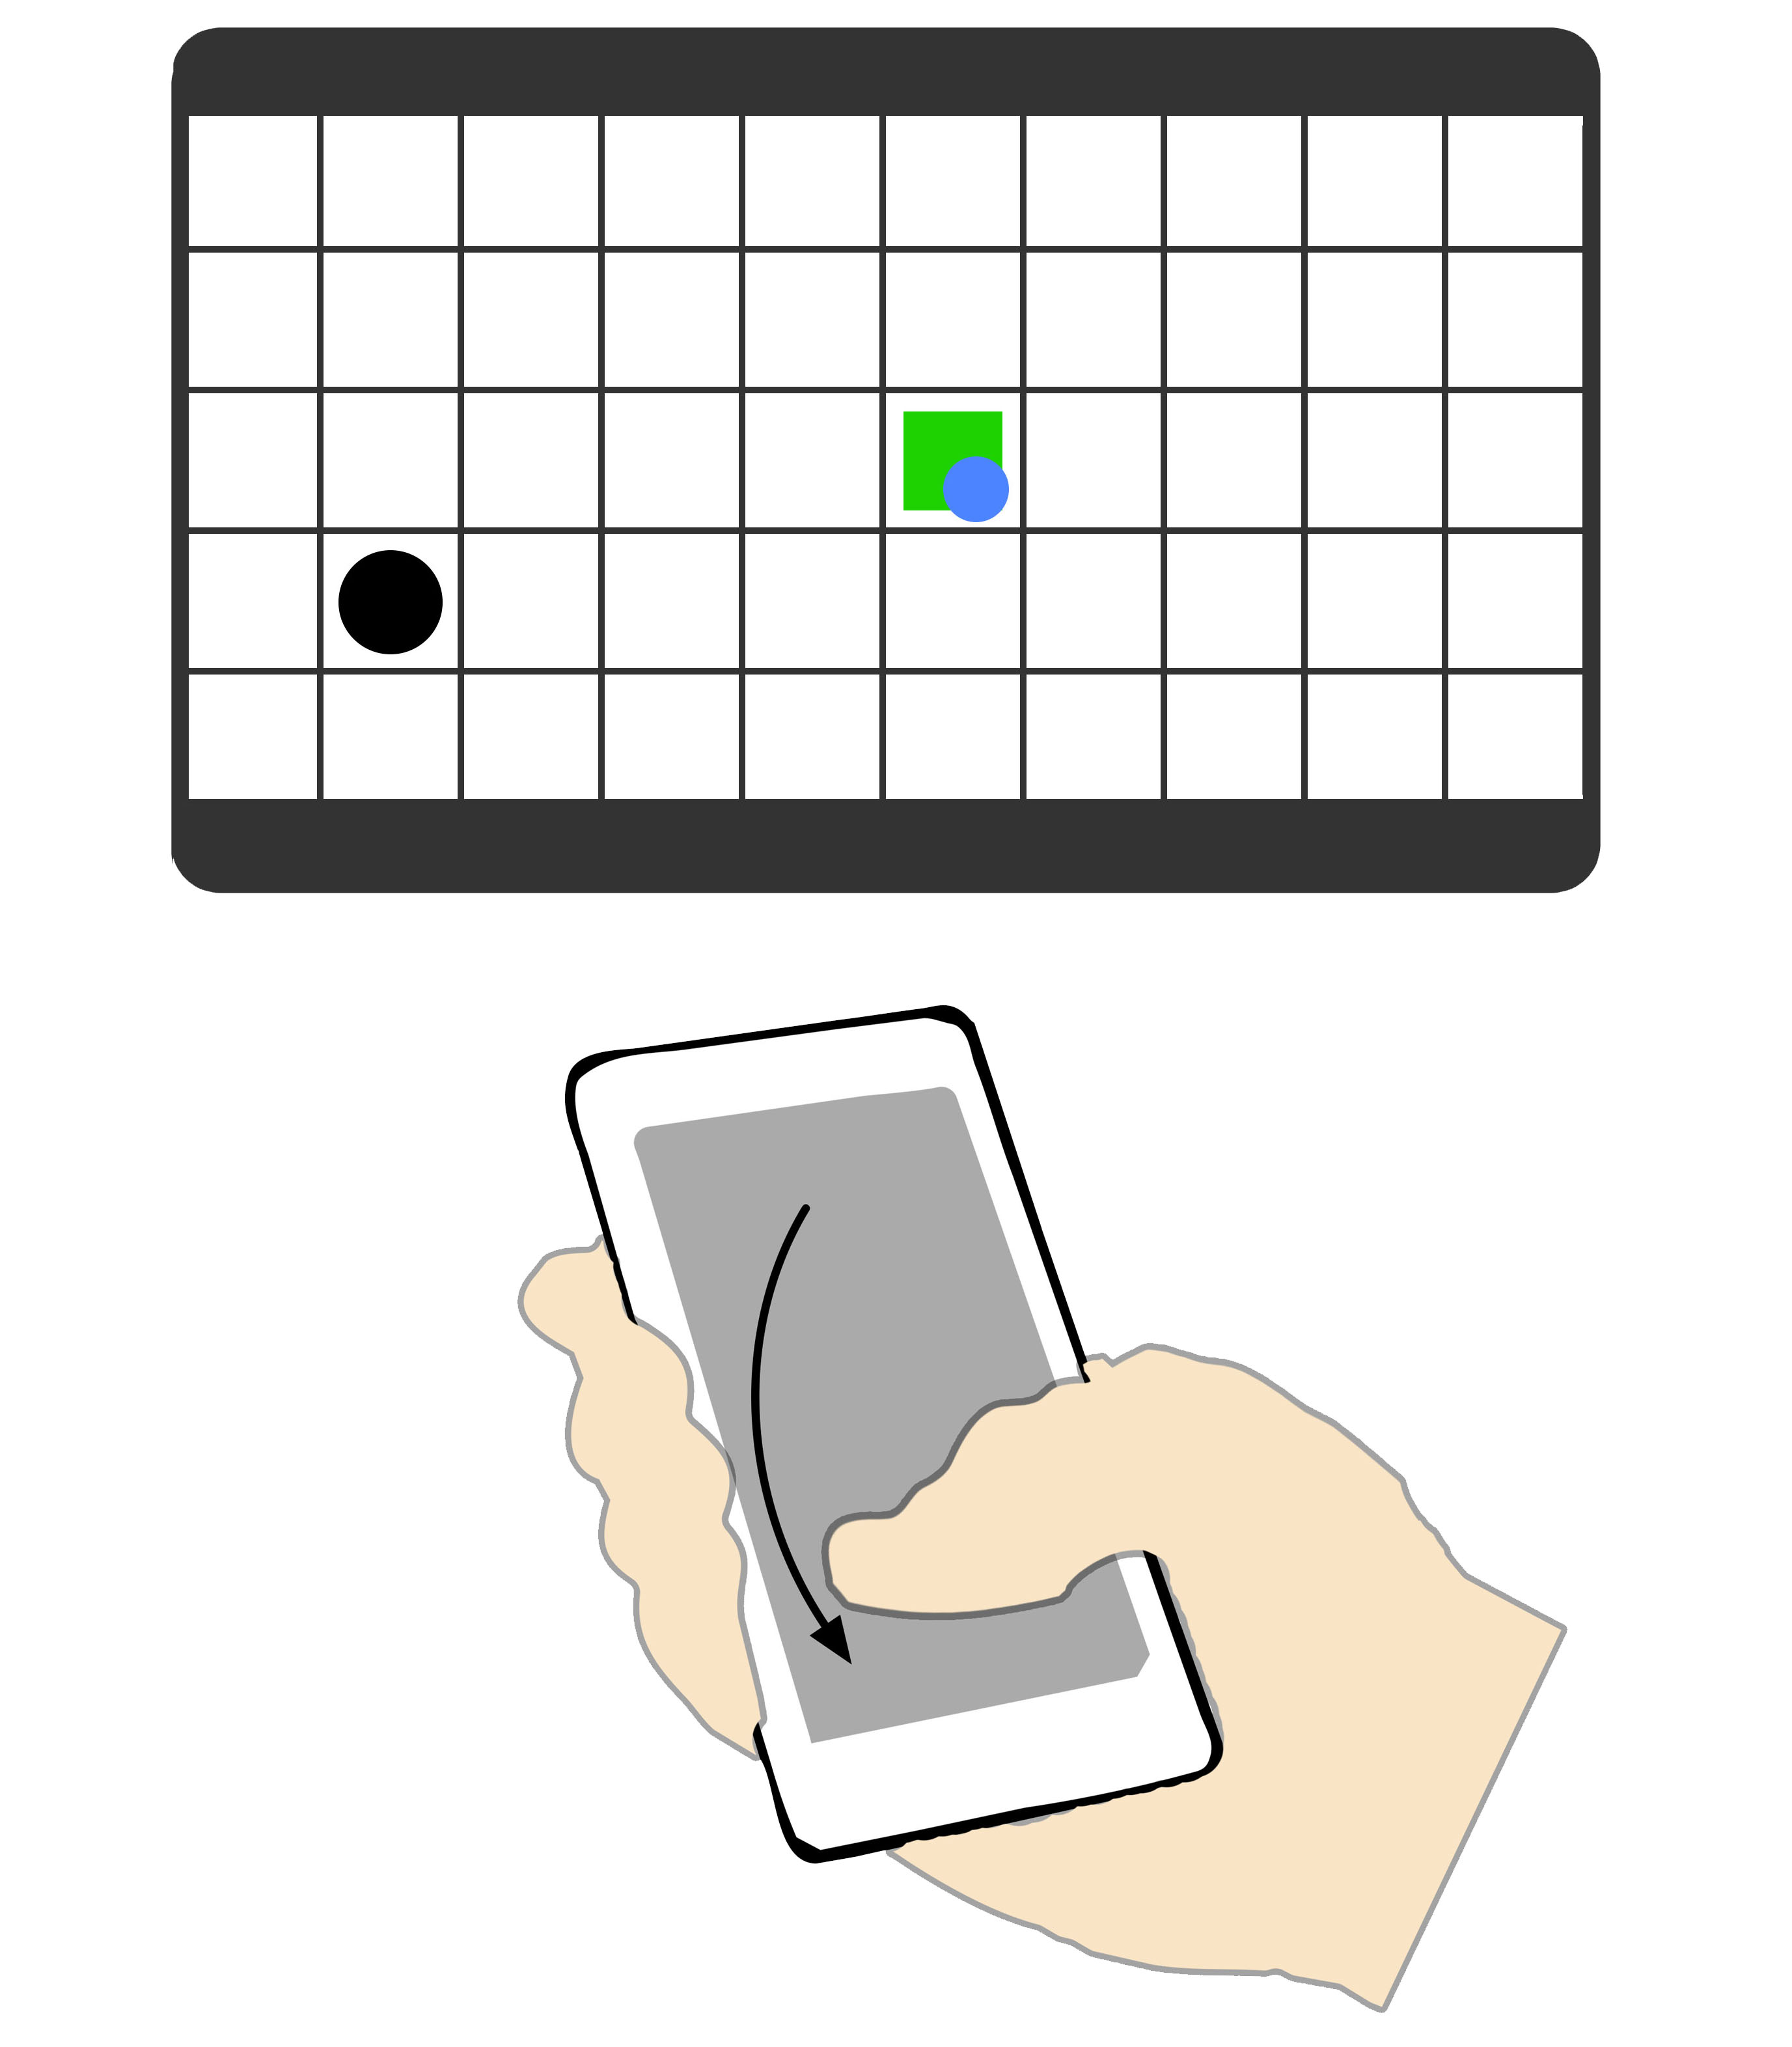
\includegraphics[width = 0.33\columnwidth]{images/techniques/swipePull3.jpg}\label{fig:swipePull3}}
	\caption{Pull swipe technique}
	\label{fig:grabTechnique}
\end{figure}

\begin{figure}[H]
	\subfloat[]{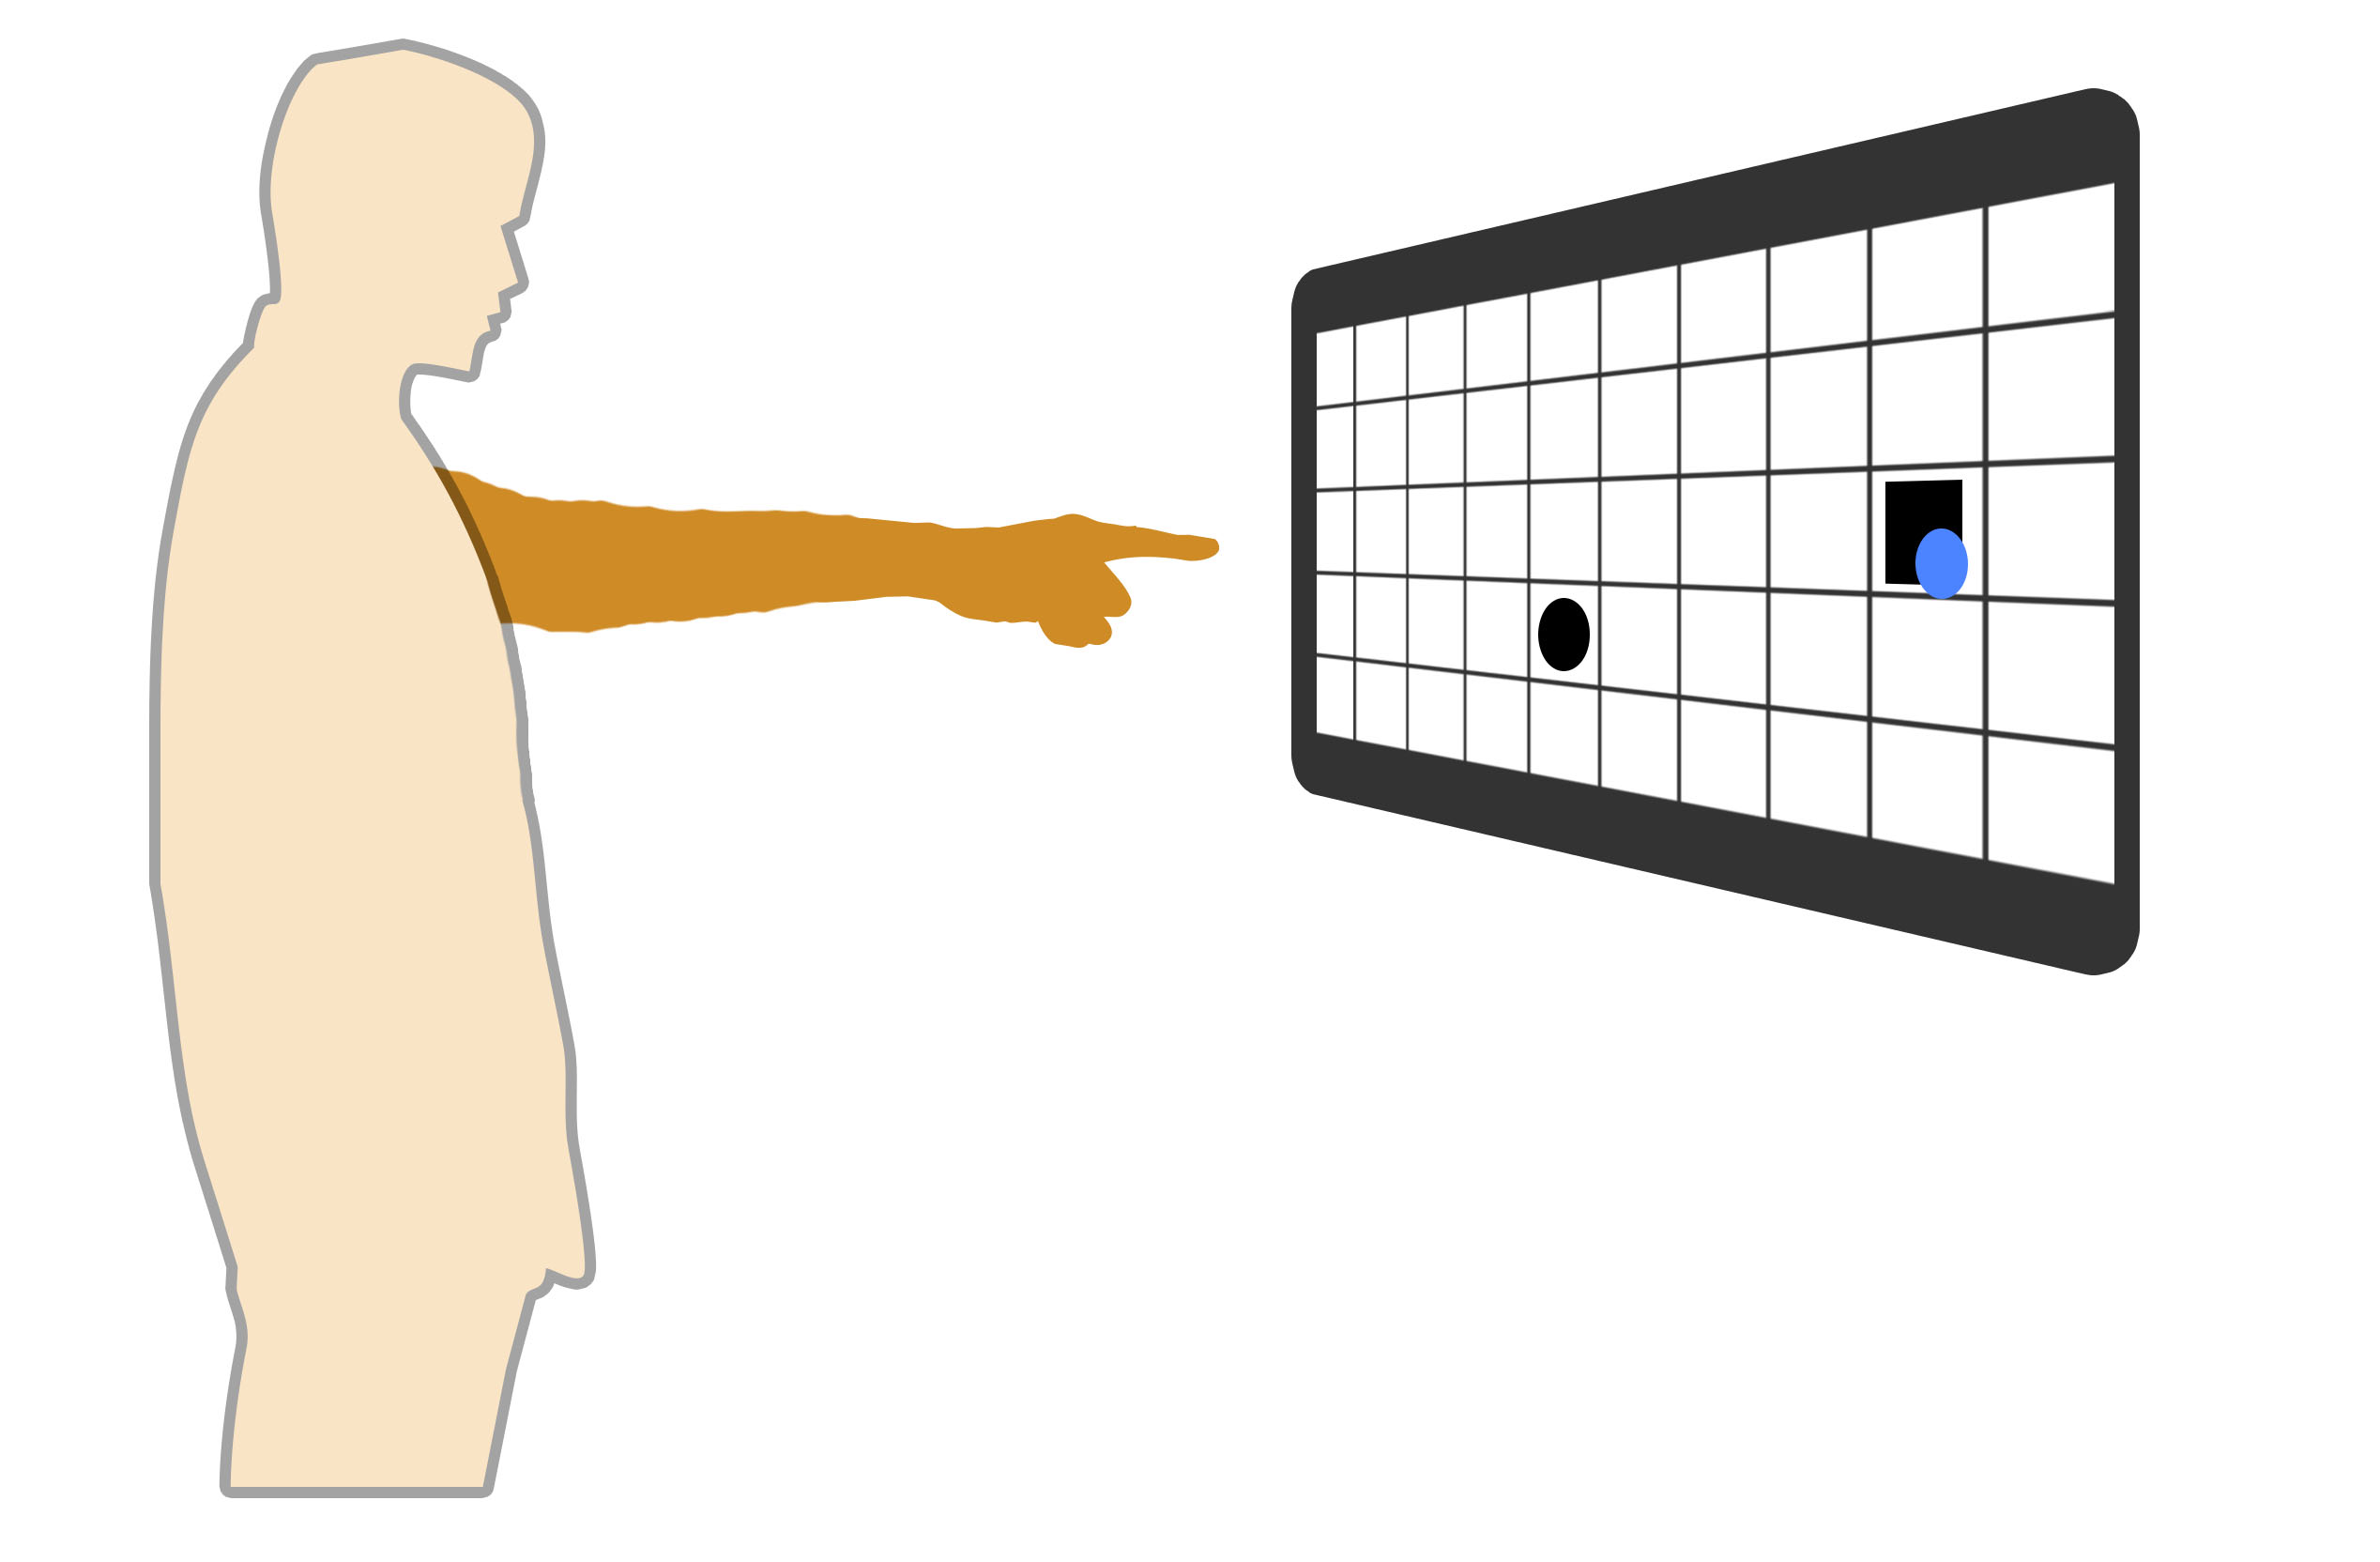
\includegraphics[width = 0.33\columnwidth]{images/techniques/throwPull1.jpg}\label{fig:throwPull1}}
	\subfloat[]{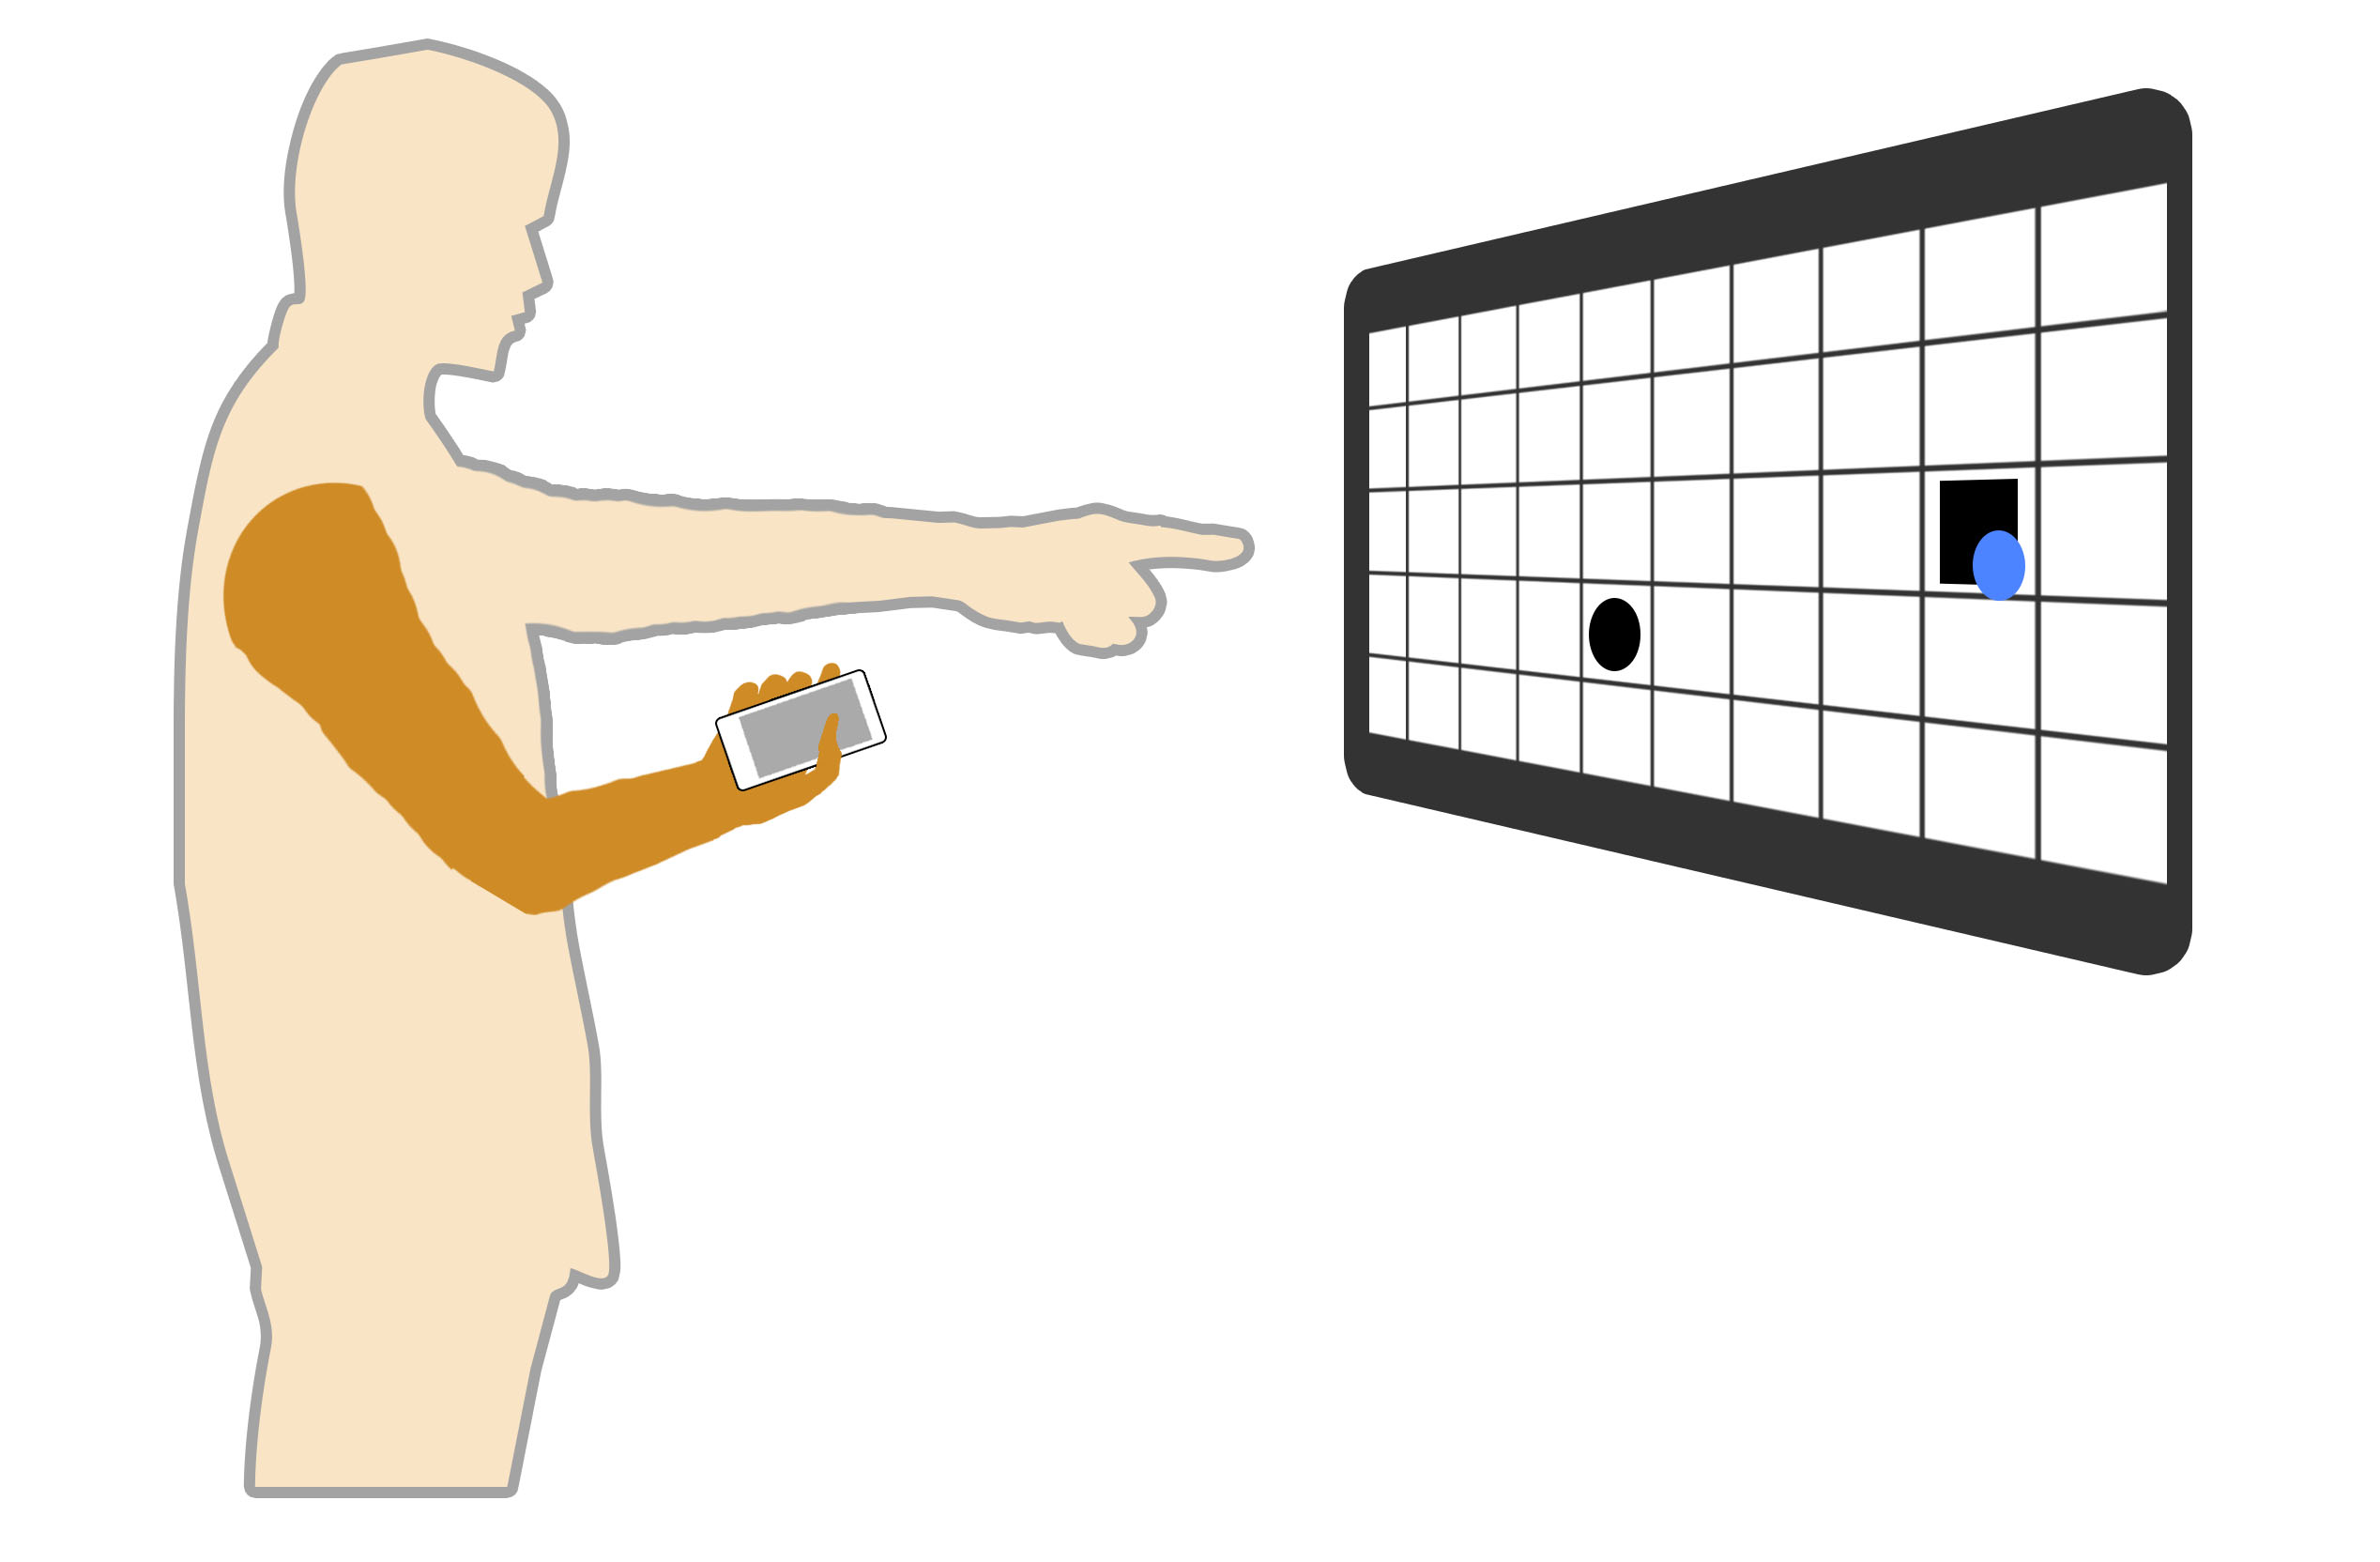
\includegraphics[width = 0.33\columnwidth]{images/techniques/throwPull2.jpg}\label{fig:throwPull2}}
	\subfloat[]{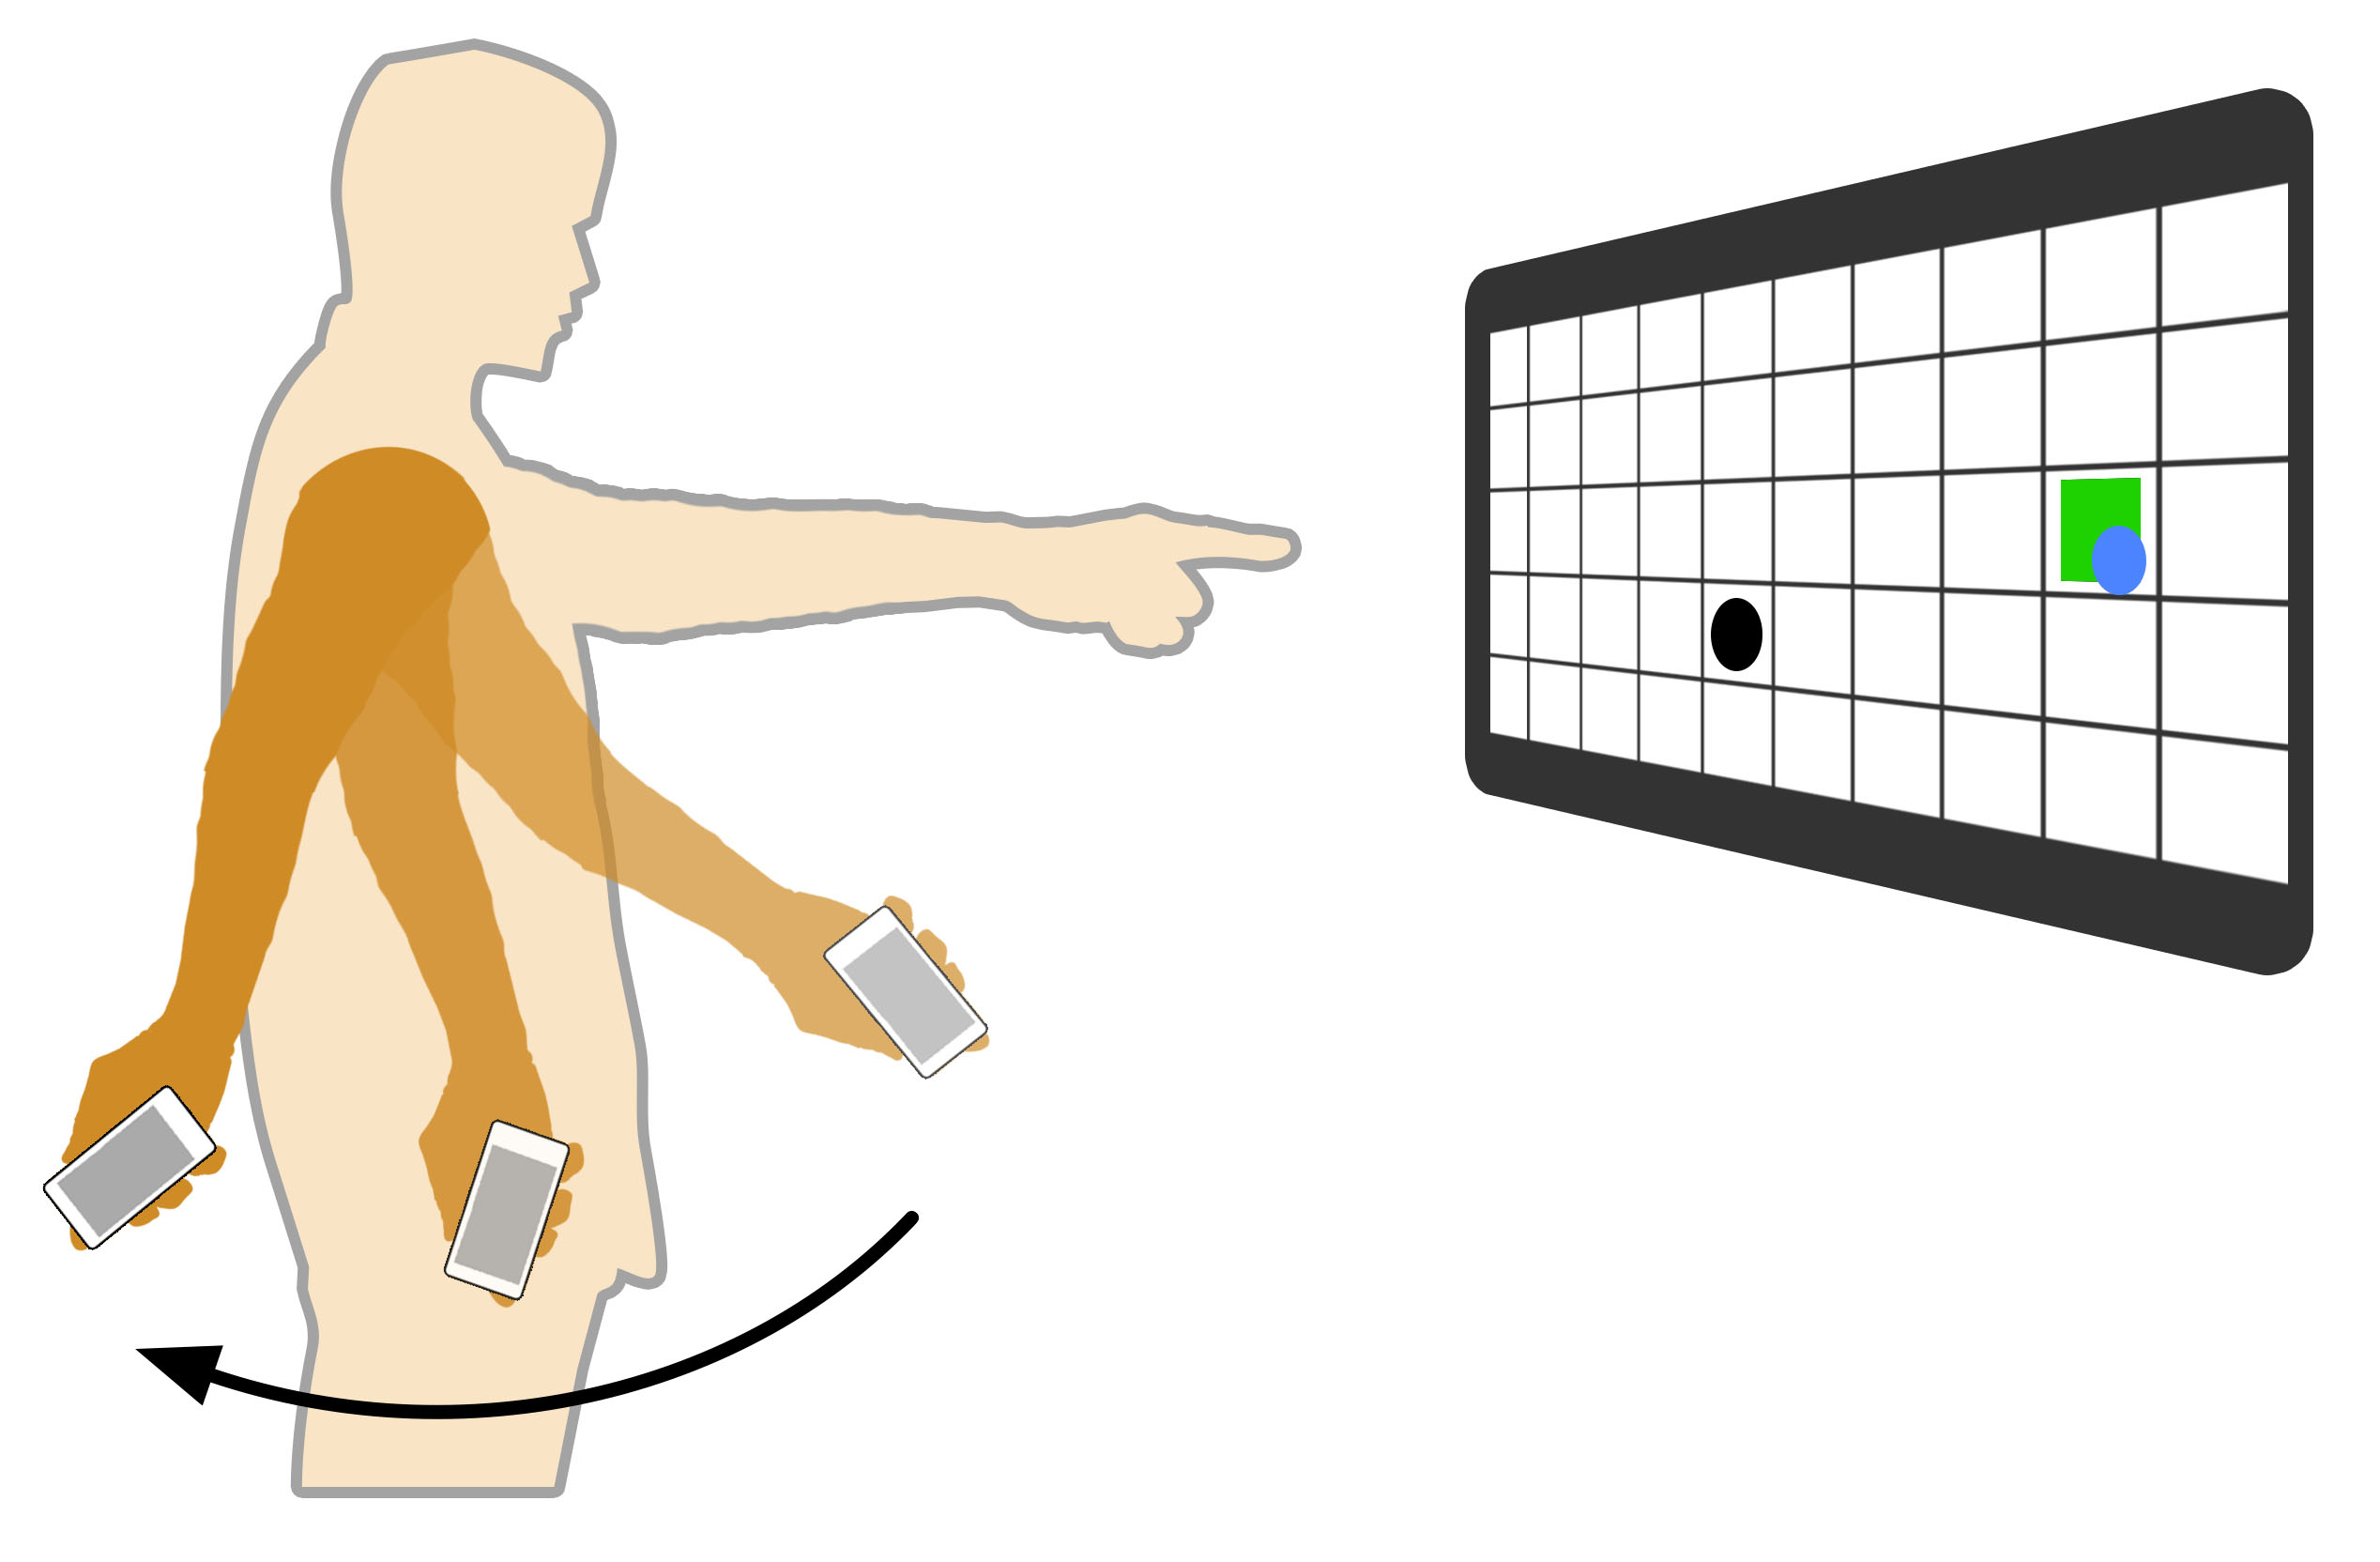
\includegraphics[width = 0.33\columnwidth]{images/techniques/throwPull3.jpg}\label{fig:throwPull3}}
	\caption{Pull throw technique}
	\label{fig:grabTechnique}
\end{figure}

\begin{figure}[H]
	\subfloat[]{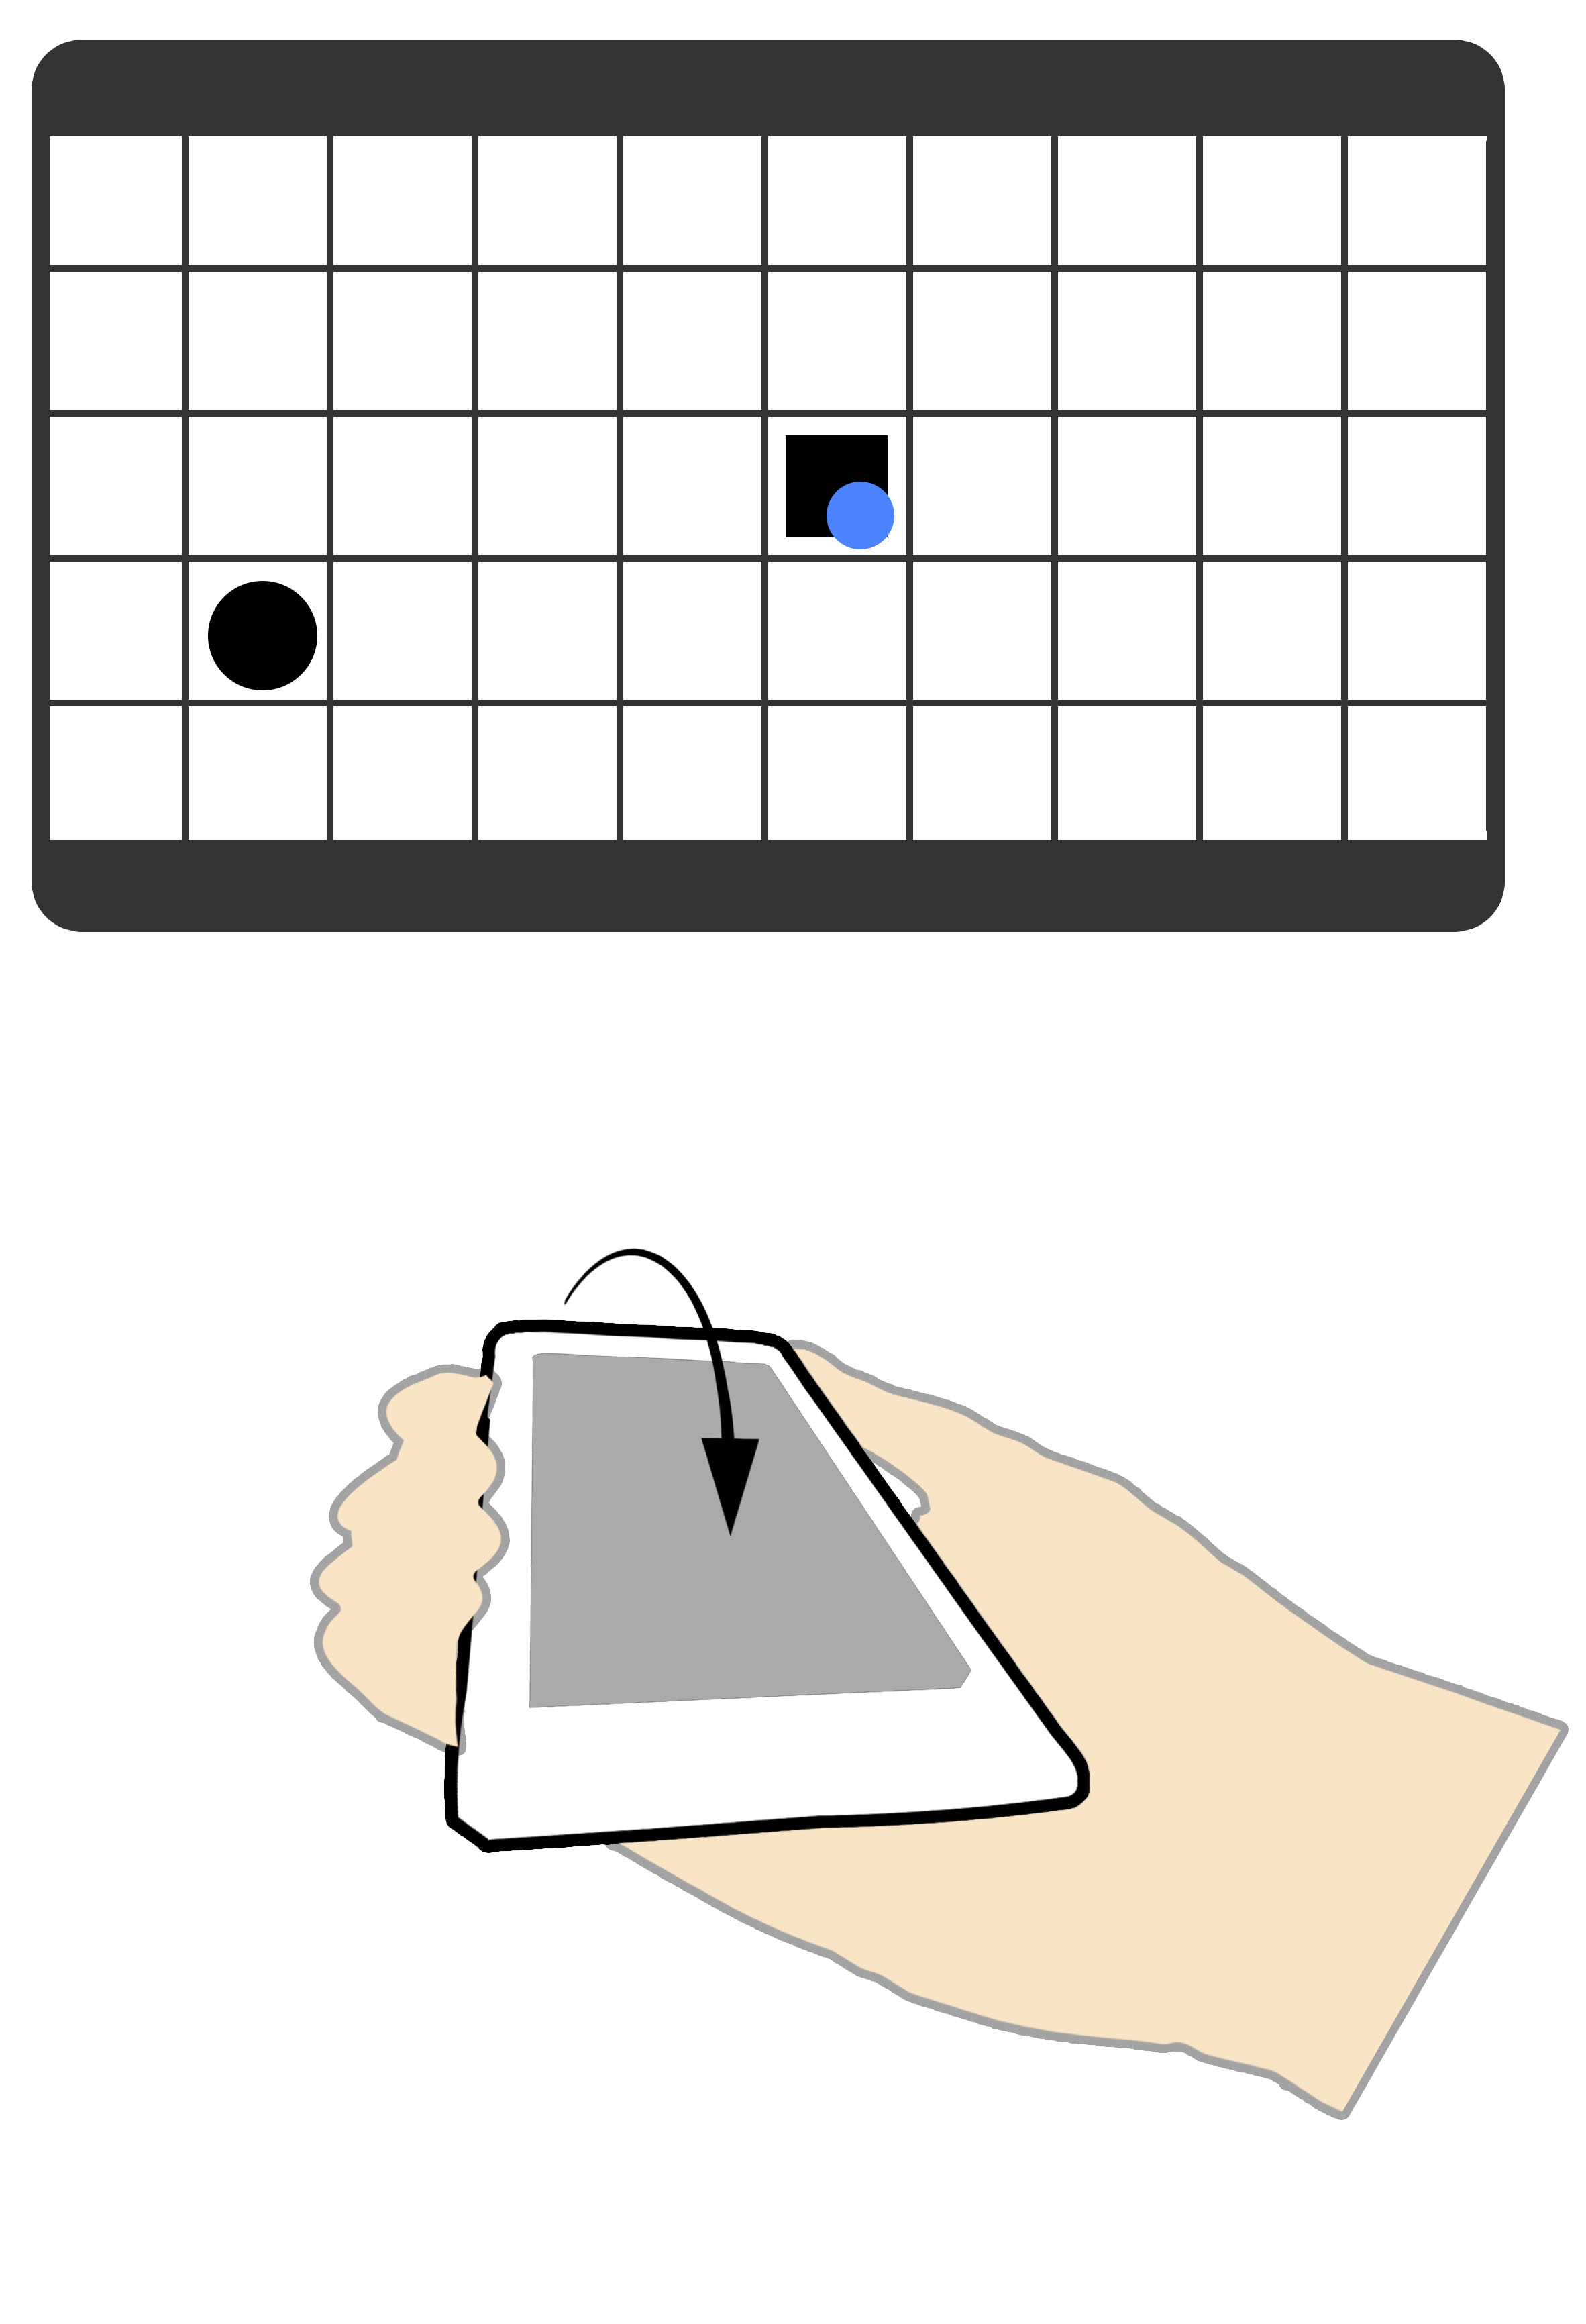
\includegraphics[width = 0.33\columnwidth]{images/techniques/tiltPull1.jpg}\label{fig:tiltPull1}}
	\subfloat[]{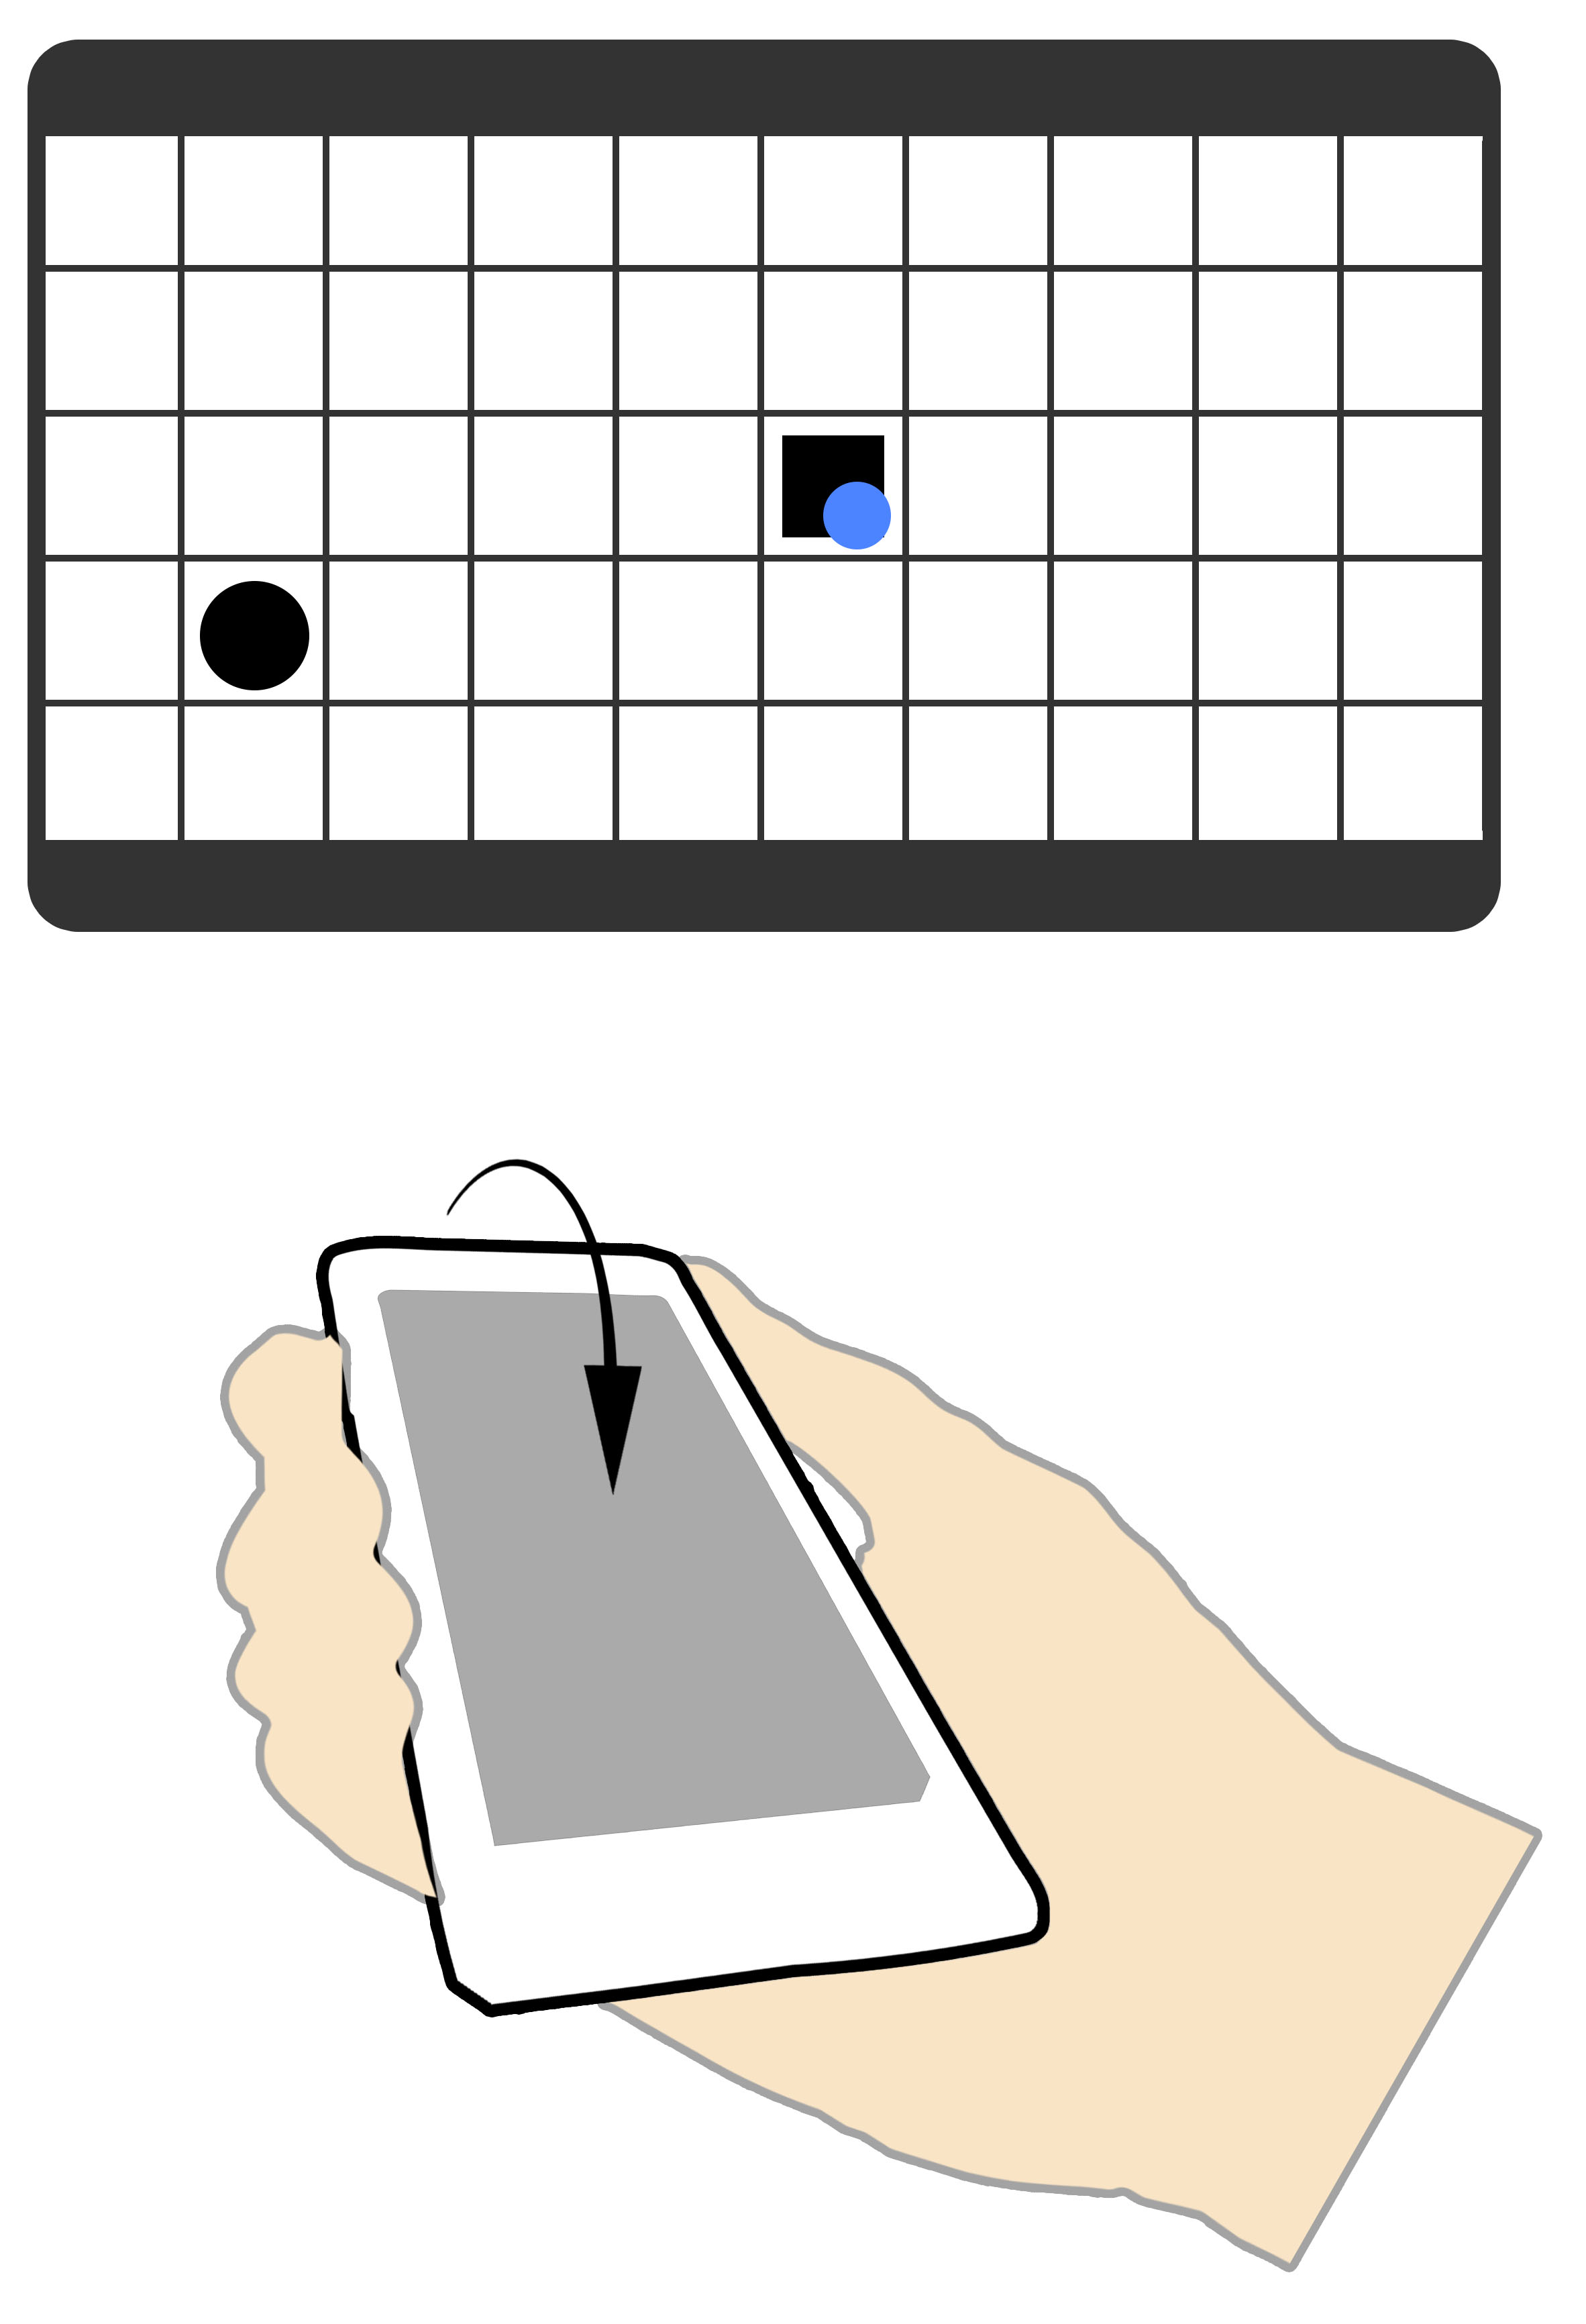
\includegraphics[width = 0.33\columnwidth]{images/techniques/tiltPull2.jpg}\label{fig:tiltPull2}}
	\subfloat[]{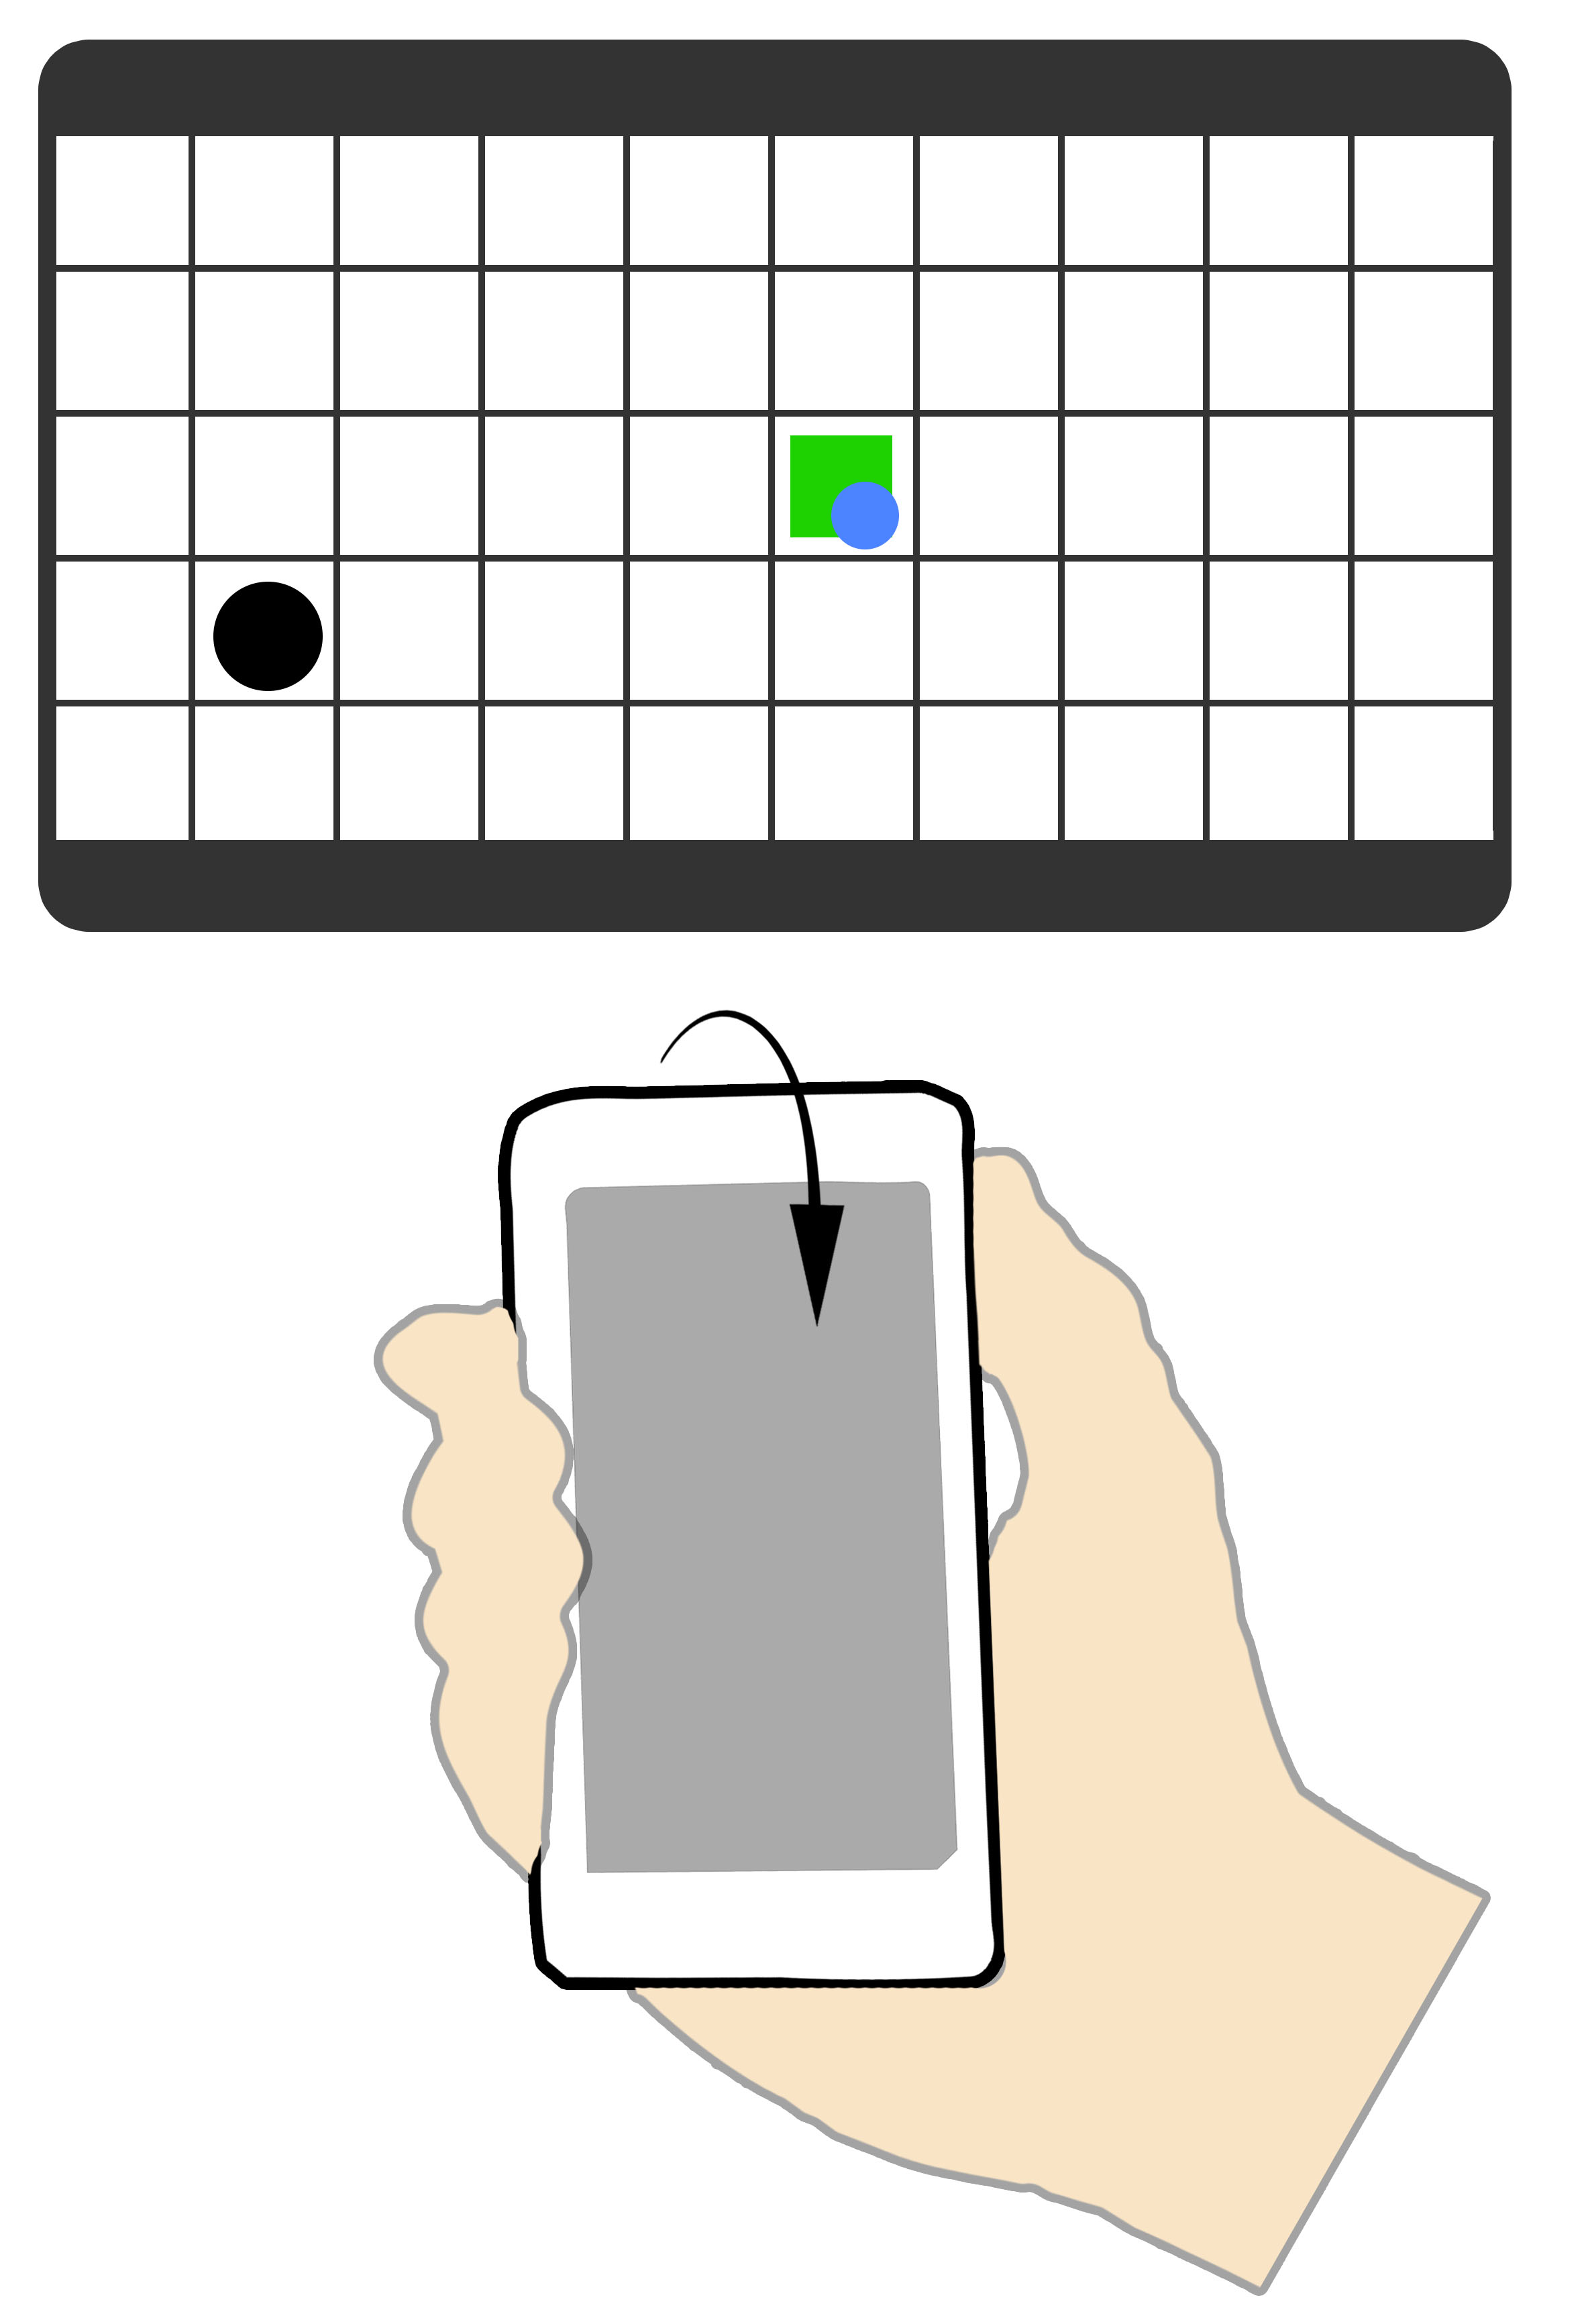
\includegraphics[width = 0.33\columnwidth]{images/techniques/tiltPull3.jpg}\label{fig:tiltPull3}}
	\caption{Pull tilt technique}
	\label{fig:grabTechnique}
\end{figure}